%%%%%%%%%%%%%%%%%%%%%%%%%%%%%%%%%%%%%%%%%%%%%%%%%%%%%%%%%%%%%%%%%%%%%%%%%%%%%%%%%%%%%%%%%
% 
% Template for Project/Internship reports, for LEEC and LETI at DEE, ISEP,
% by Vitor M. R. Cunha - v1.1, Jul 2021
% Suggestions and comments are welcomed (vrc at isep dot ipp dot pt).
%
% Template provided as is, NO SUPPORT will be given.
% NO questions related to LaTeX will be answered, go to
% https://ftp.eq.uc.pt/software/TeX/info/lshort/english/lshort.pdf, or search the web.
%
% The DEE document class uses the LaTeX book base class, the original work credits are
% in the document class file.
%
% Overleaf template direct link:
% 
% or go to https://www.overleaf.com/gallery/, and search for: ISEP LEEC
%
%%%%%%%%%%%%%%%%%%%%%%%%%%%%%%%%%% MAIN SETTINGS %%%%%%%%%%%%%%%%%%%%%%%%%%%%%%%%%%%%%%%%

\documentclass[
LETI,			% Use this option to select your DEE degree, options: LEEC, LETI
portuguese,		% Select document language, options: portuguese or english
%draft,			% Uncomment for draft mode (no pictures, no links, overfull hboxes) 
]{DEEclass}

% Use the 'preamble.tex' file (root folder) do add packages and macros. Keep your main.tex file clean.

% FYI, the following packages are preloaded with the document class:
% longtable, xcolor, graphicx, booktabs, caption, csquotes, hyperref,
% calc, listings, datetime2, siunitx, geometry, enumitem

%%%%%%%%%%%%%%%%%%%%%%%%%%%%%%%%%%%%%%%%%%%%%%%%%%%%%%%%%% extra packages
\usepackage{amsmath}		% the main package in the AMS-LATEX distribution
\usepackage{amsfonts}		% extended set of fonts for use in mathematics
\usepackage{amssymb}		% adds new symbols to be used in math mode
\usepackage{mathrsfs}		% math fonts, e.g., Laplace
\usepackage{float}			% provides the H float modifier option
\usepackage{multirow}		% tables \multirow command
\usepackage{subcaption}		% enables subfigures
\usepackage{lscape}			% for landscape mode
\usepackage{verbatim}		% new verbatim environment, \begin{comment}...\end{comment}, \verbatiminput

%add extra packages if needed here

%%%%%%%%%%%%%%%%%%%%%%%%%%%%%%%%%%%%%%%%%%%%%%%%%%%%%%%%%% temp packages
\usepackage{lipsum}						% for fake text
%\usepackage[textsize=tiny]{todonotes}   % enable To-do notes, use the option "disable" to hide all notes, usage \todo{}

%\usepackage{draftwatermark}			% prints a watermark overlay, uncomment if needed
%\SetWatermarkText{**DRAFT**}
%\SetWatermarkScale{1}
%\SetWatermarkColor[gray]{0.8}

%%%%%%%%%%%%%%%%%%%%%%%%%%%%%%%%%%%%%%%%%%%%%%%%%%%%%%%%%% settings
\AtBeginDocument{					% Rendered PDF metadata:
\hypersetup{pdftitle=\ttitle} 		% Sets the PDF title to your dissertation title
\hypersetup{pdfauthor=\authorname} 	% Sets the PDF author to your name
}

%%%%%%%%%%%%%%%%%%%%%%%%%%%%%%%%%%%%%%%%%%%%%%%%%%%%%%%%%% user defined macros

%....








		 

%%%%%%%%%%%%%%%%%%%%%%%%%%%%%%%% REPORT INFORMATION %%%%%%%%%%%%%%%%%%%%%%%%%%%%%%%%%%%%%

\reporttitle{Developing applications with Ballerina} % Your report title

%\reportsubtitle{Com um Subtítulo se Necessário} % and subtitle, uncomment if needed
%\subdate{Janeiro, 2021} % Uncomment for a static submission date, or leave it as a comment for automatic date (month+year) 

\author{Tiago Nora}	% Your name
\studentnumber{1201050}	% Your student number
\studentemail{1201050@isep.ipp.pt}	% Your student email address  

\advisor{Nome do Orientador}{xxx@isep.ipp.pt}	% Your ISEP advisor name and email
\coadvisor{Nome do Coorientador}{xxx@isep.ipp.pt}	% Your ISEP co-advisor name and email, comment this line if not needed
\company{Nome da Empresa, Lda.}	% The company name where you developed your work, comment this line if not needed
\supervisor{Nome do Orientador da Empresa}{xxx@emailaddress.com} % Your company supervisor name, comment this line if not needed

%%%%%%%%%%%%%%%%%%%%%%%%%%%%% USER DEFINED LISTS %%%%%%%%%%%%%%%%%%%%%%%%%%%%%%%%%%%%%%%%
\makeglossaries						% Consider the following files in the 'front' folder:
%----------------------------------------------------------------------------------------
%	GLOSSARY
%----------------------------------------------------------------------------------------

% Only the used entries will be displayed in the printed list, ie, you need to used a term at least once
% In italic if not in the main document language

% terms definition usage:
% \newglossaryentry{<tag>}{name={<term>},description={<description of the term>}}

\newglossaryentry{gloss}{
name={glossário}, 
description={é uma lista alfabética de termos de um determinado domínio de conhecimento com a definição desses mesmos termos.},
}

\newglossaryentry{pack}{
name={\textit{package}}, 
description={é um ficheiro ou conjunto de ficheiros que contêm comandos \LaTeX{} extra que adicionam novas funcionalidades de estilo ou modificam aquelas já existentes.},
sort={package}	%needed for sorting when using LaTeX commands in the 'name' field
}

\newglossaryentry{lipsum}{
name={\textit{Lorem Ipsum}}, 
description={é uma sequência de palavras, geralmente latinas, utilizada para preencher o espaço destinado a texto numa publicação, por forma a testar as opções de formatação e edição e o arranjo dos elementos gráficos antes da inserção do conteúdo.},
sort={Lorem Ipsum}
}
			% Edit to define your glossary entries list
%----------------------------------------------------------------------------------------
%	ACRONYMS LIST
%----------------------------------------------------------------------------------------

% Only the used entries will be displayed in the printed list, ie, you need to used a acronym at least once
% Full name in italic if not in the main document language

%acronym definition usage:
%\newacronym{<tag>}{<acronym>}{<full name>}

\newacronym{wys}{WYSIWYG}{\textit{What You See Is What You Get}}
\newacronym{dee}{DEE}{Departamento de Engenharia Electrotécnica}
\newacronym{api}{API}{\textit{Application Programming Interface}}
\newacronym{ascii}{ASCII}{\textit{American Standard Code for Information Interchange}}
\newacronym{html}{HTML}{\textit{HyperText Markup Language}}
\newacronym{isep}{ISEP}{Instituto Superior de Engenharia do Porto}
\newacronym{leec}{LEEC}{Licenciatura em Engenharia Eletrot\'{e}cnica e de Computadores}
\newacronym{leti}{LETI}{Licenciatura em Engenharia de Telecomunicações e Informática}
\newacronym{usb}{USB}{\textit{Universal Serial Bus}}
\newacronym{pdf}{PDF}{\textit{Portable Document Format}}
			% Edit to define your acronyms entries list
%----------------------------------------------------------------------------------------
%	SYMBOLS LIST
%----------------------------------------------------------------------------------------

% terms definition usage:
% \newglossaryentry{<tag>}{
% name={<symbol>},
% sort={<text for the alphabetical sorting>},
% description={<description of the symbol>},
% unit={<units to display>},
% type=symbolslist}

\newglossaryentry{f}{
name={\ensuremath{f}},
sort={f},
description={força},
unit=\si{\newton},
type=symbolslist}

\newglossaryentry{i}{
name={\ensuremath{i}},
sort={i},
description={corrente},
unit=\si{\ampere},
type=symbolslist}

\newglossaryentry{m}{
name=\ensuremath{M},
sort={m},
description={massa},
unit=\si{\kilogram},
type=symbolslist}

\newglossaryentry{p}{
name=\ensuremath{P},
sort={p},
description={potência},
unit=\si{\watt},
type=symbolslist}

\newglossaryentry{theta}{
name=\ensuremath{\theta},
sort={z1},
description={deslocamento angular},
unit=\si{\radian},
type=symbolslist}

\newglossaryentry{omega}{
name=\ensuremath{\omega},
sort={z2},
description={velocidade angular},
unit=\si{\radian\per\second},
type=symbolslist}

\newglossaryentry{x}{
name=\ensuremath{x},
sort={x},
description={deslocamento},
unit=\si{\meter},
type=symbolslist}

% Greek: alpha,beta,gamma,delta,epsilon,zeta,eta,theta,iota,kappa,lambda,mu,nu,xi,omikron,pi,rho,sigma,tau,upsilon,phi,chi,psi,omega
				% Edit to define your symbols entries list

%%%%%%%%%%%%%%%%%%%%%%%%%%%%%%%%%%%%%%%%%%%%%%%%%%%%%%%%%%%%%%%%%%%%%%%%%%%%%%%%%%%%%%%%%
\begin{document}
\frontmatter

%----------------------------------------------------------------------------------------
%	TITLE PAGES
%----------------------------------------------------------------------------------------
\pagestyle{plain} % Default to the plain heading style until the thesis style is called for the body content
\printcoverpage
\printaftercoverpage
\cleardoublepage















%%%%%%%%%%%%%%%%%%%%%%%%%%%%%%%%%%% FRONTMATTER %%%%%%%%%%%%%%%%%%%%%%%%%%%%%%%%%%%%%%%%%
% Consider the following front matter sections provided as separate files in the 'front' folder.
% Comment the lines regarding the sections you will not use, or edit the file contents as needed

%----------------------------------------------------------------------------------------
%	DEDICATION
%----------------------------------------------------------------------------------------

\dedicatory{
(Opcional) Poderá usar esta secção para dedicar o trabalho a alguém\ldots
} 
		% Edit if you want to dedicate your work to someone, or comment this line if not used
%----------------------------------------------------------------------------------------
%	ACKNOWLEDGEMENTS
%----------------------------------------------------------------------------------------

\begin{acknowledgements}

Eu gostaria de agradecer à minha orientadora Isabel Azevedo por toda a orientação e por estar sempre disponível para ajudar durante o percurso do desenvolvimento deste trabalho. As reuniões semanais ajudaram muito, não só para esclarecer as minhas dúvidas, mas como para discutir como poderia melhor o meu relatório.

Também gostaria de agradecer aos meus familiares, que me forneceram todos os materiais necessários para eu ter sucesso na vida e aos meus amigos pelo apoio demonstrado.

E por fim, gostaria de agradecer a todos os meus colegas e docentes que passaram pela minha académica no ISEP.

\end{acknowledgements}
	% Edit to add the due acknowledgements, or comment this line if not used
%----------------------------------------------------------------------------------------
%	ABSTRACT PAGES
%----------------------------------------------------------------------------------------

% IMPORTANT NOTE: the abstract must always be written in two languages. If the report
% is written in Portuguese you have selected 'portuguese' as the language in the document class.
% Therefore, the portuguese version of the abstract must come first, so write it in the
% below area denoted by 'MAIN LANGUAGE ABSTRACT'. The english version follows in the
% 'SECOND LANGUAGE ABSTRACT' section.
% If the report is written in English, first will come the abstract in English
% ('MAIN LANGUAGE ABSTRACT') and then in Portuguese ('SECOND LANGUAGE ABSTRACT').

\begin{abstract}
%%%%%%%%%%%%%%%%%%%%%%%%%%%%%% MAIN LANGUAGE ABSTRACT %%%%%%%%%%%%%%%%%%%%%%%%%%%%%%%%%%

Aqui deverá ser apresentado o resumo de todo o trabalho efetuado. Esta secção não deverá exceder uma página.

Deve contextualizar o problema que pretende resolver ou a hipótese que irá formular, procure evidenciar as vantagens e desvantagens (se as houver) da solução encontrada, como também a forma através da qual a solução/hipótese foi validada. Neste último ponto, deverá referir-se aos desenvolvimentos efetuados, e à forma como validou (conformidade) e avaliou (desempenho) a solução encontrada.

O documento deve conter sempre duas versões do resumo: uma primeira no idioma do texto principal e a segunda num outro idioma. Este \textit{template} assume que os dois idiomas em consideração são sempre Português e Inglês, assim, a classe irá colocar os cabeçalhos respetivos de acordo com o idioma selecionado nas opções da classe no ficheiro \file{main.tex}. 

%----------------------------------------------------------------------------------------

\vspace*{10mm} 
\noindent
\textbf{\keywordslabel}: Lista, separada por vírgulas, de palavras, frases, ou acrónimos chave no âmbito do trabalho descrito neste texto. 

%%%%%%%%%%%%%%%%%%%%%%%%% END OF THE MAIN LANGUAGE ABSTRACT %%%%%%%%%%%%%%%%%%%%%%%%%%%%%%
\end{abstract}
\begin{secondlangabstract}
%%%%%%%%%%%%%%%%%%%%%%%%%%%%%% SECOND LANGUAGE ABSTRACT %%%%%%%%%%%%%%%%%%%%%%%%%%%%%%%%%%

The summary of all the developed work should be presented here. This section should not exceed one page.

Start the abstract with the contextualization of the problem you intend to solve or the hypothesis you will formulate. Try to highlight the advantages and disadvantages (if any) of the solution found, as well as the way in which the solution/hypothesis was validated. In this last point, you should refer to the developments made, and to the way you validated (compliance) and evaluated (performance) the solution found.

The document must always contain two versions of the abstract: a first in the language of the main text and the second one in another language. This template assumes that the two languages are always Portuguese and English, therefore, the class will place the correct section headers according to the language selected in the class options in the \file{main.tex} file.


%----------------------------------------------------------------------------------------

\vspace*{10mm} 
\noindent
\textbf{\keywordslabel}: Comma separated list of words, phrases, or key acronyms within the scope of your developed work. 

%%%%%%%%%%%%%%%%%%%%%%%%%% END OF THE SECOND LANGUAGE ABSTRACT %%%%%%%%%%%%%%%%%%%%%%%%%%%%%
\end{secondlangabstract}

			% Edit the file to write the document Abstract. Two languages are always required.
%----------------------------------------------------------------------------------------
%	FONTMATTER LISTS
%----------------------------------------------------------------------------------------
\pdfbookmark[0]{\contentsname}{toc}
\tableofcontents 	
\glsresetall
%----------------------------------------------------------------------------------------

% Of the following lists, comment the ones you will not use in your document

\listoffigures 			% Prints the list of figures

\listoftables 			% Prints the list of tables

\printlistoflistings	% Prints the list of listings (source code segments)

\printlistofterms		% Prints the list of USED terms (glossary)

\printlistofacronyms{XXXXXXXXI} % Prints the list of USED acronyms
% Change the argument with random letters to adjust the left alignment of the acronyms full name column

\printlistofsymbols		% Prints the list of ALL defined symbols
	% Edit the file to select the lists to be shown (figures, tables, source code segments, glossary, acronyms, symbols)

%%%%%%%%%%%%%%%%%%%%%%%%%%%%%%%%%%% MAINMATTER %%%%%%%%%%%%%%%%%%%%%%%%%%%%%%%%%%%%%%%%%
\mainmatter 
\pagestyle{thesis} 				

% Include the chapters of the document as separate files from the 'chapters' folder

%%%%%%%%%%%%%%%%%%%%%%%%%%%%%%%%%%%% Chapter Template

\chapter{Introdução} 	% Main chapter title
\label{Chapter1} 		% For referencing the chapter elsewhere, usage \ref{Chapter1}

%%%%%%%%%%%%%%%%%%%%%%%%%%%%%%%%%%%%

Este documento pretende guiar o Estudante na elaboração do relatório de Projeto/Estágio, do 3º ano da \ac{leec} e da \ac{leti}, do \ac{dee}, do \ac{isep}.

O autor deverá ter em consideração as seguintes regras gerais na elaboração do documento:

\begin{itemize}
	\item É fundamental refletir, antes de escrever, sobre a substância do que se pretende transmitir.
	\item Deve organizar o texto evitando a excessiva divisão do mesmo em tópicos que supostamente se enquadram no tema principal da secção a que pertencem. A excessiva especialização pode ser reveladora de falta de conhecimento e/ou reflexão. Neste sentido, deve, antes de iniciar a escrita, exercitar-se em refinar a organização do texto com o intuito de evitar que existam mais do que 2 níveis de ``profundidade'' em cada secção (respetivamente, subsecção e sub-subsecção). Note que o número de capítulos, secções e subsecções do presente documento não é vinculativo nem mesmo indicativo, apenas serve os propósitos do mesmo.
	\item O documento deve ser redigido em português ou inglês com um estilo adequado (evite o tom coloquial, lugares comuns e chavões) e correto do ponto de vista gramatical (quer do ponto de vista sintático quer semântico).
	\item Tenha especial cuidado com o uso de adjetivos (facilmente conduzem ao exagero), advérbios (nada, ou quase nada, acrescentam) e sinais de pontuação (em especial o uso correto das vírgulas).
	\item O estilo adotado para a redação deve ser coerente com as exigências de um trabalho científico encontrado em publicações impressas.
	\item De uma forma genérica deve usar a 3ª pessoa do singular (eventualmente do plural), exceção feita aos locais onde tal é claramente desajustado, por exemplo, na secção dos agradecimentos.
	\item Usar o estilo \textit{itálico} sempre que são utilizados termos em línguas diferentes da língua adotada no relatório.
	\item O uso de acrónimos implica que na 1ª vez que são utilizados se apresentem por extenso, colocando entre parênteses a respetiva sigla que se passará a usar. No entanto, é sempre possível, mais à frente no texto, e por uma questão de legibilidade, repetir o significado do acrónimo. Todos os acrónimos devem ser apresentados por ordem alfabética na secção ``Lista de Acrónimos''.
	\item O uso correto de unidades, seus múltiplos e submúltiplos.
	\item As imagens e tabelas devem, por princípio, aparecer no topo ou no fundo da página. A legendas surgem imediatamente após as figuras e listagens. No caso das tabelas as legendas antecedem as mesmas.
	\item Todas as figuras, tabelas e restantes listagens devem ser mencionadas no texto por forma a que fiquem enquadradas nas ideias transmitidas pelo autor. Esta referência, regra geral, deverá ser feita antes da ocorrência da figura, tabela ou listagem.
	\item Deve indicar ao longo do texto as referências documentais usadas, em especial nas citações (puras ou literais), assinaladas com a utilização de aspas, como também no caso de reutilização de gráficos, figuras, tabelas, fórmulas, etc., de outras fontes.
\end{itemize}

De uma forma já mais específica, neste primeiro capítulo obrigatório (``Introdução'') o autor deve:

\begin{itemize}
	\item contextualizar a proposta de trabalho no âmbito da empresa, de um outro trabalho já realizado, do ponto de vista científico e/ou tecnológico, etc.,
	\item apresentar de forma clara os objetivos que se propõe atingir,
	\item descrever de forma sucinta, mas objetiva, a solução preconizada ou a hipótese colocada,
	\item apresentar de forma resumida, mas clara, os desenvolvimentos efetuados,
	\item identificar como foi validada e avaliada a solução encontrada,
	\item descrever a organização do documento.
\end{itemize}

Sem ser exigida nenhuma organização em particular para este capítulo, são indicadas a título de exemplo 4 secções (com texto \gls{lipsum}) que podem ser incorporadas nesta parte do documento: Contextualização, Descrição do Projeto, Calendarização e Organização do Relatório. 	

%%%%%%%%%%%%%%%%%%%%%%%%%%%%%%%%%%%% SECTION 1

\section{Contextualização}
\label{sec:Ch1.1}

\lipsum[1] % inserts fake text, to be removed in your dissertation

%%%%%%%%%%%%%%%%%%%%%%%%%%%%%%%%%%%% SECTION 2

\section{Descrição do Projeto}
\label{sec:Ch1.2}

\lipsum[2]

%%%%%%%%%%%%%%%%%%%%%%%%%%%%%%%%%%%% SUBSECTION 1

\subsection{Objetivos}
\label{sub:Ch1.2.1}

\lipsum[2]

%%%%%%%%%%%%%%%%%%%%%%%%%%%%%%%%%%%% SECTION 3

\section{Calendarização}
\label{sec:Ch1.3}

\lipsum[1]
% you could use the pgfgantt package: https://ctan.org/pkg/pgfgantt


%%%%%%%%%%%%%%%%%%%%%%%%%%%%%%%%%%%% SECTION 4

\section{Organização do Relatório}
\label{sec:Ch1.4}

\lipsum[2]




% Chapter 2

\chapter{Como Usar o \textit{Template} \LaTeX{} para Relatórios de PESTA}	%The main chapter title
\chaptermark{O \textit{Template}}	%Short version for page header. Comment if not needed
\label{Chapter2}	%For referencing the chapter elsewhere, use \ref{Chapter2} 

%%%%%%%%%%%%%%%%%%%%%%%%%%%%%%%%%%%%

A opção pelo \LaTeX{} para elaborar o relatório favorece o aspeto gráfico do documento final, mas um documento visualmente bonito não substitui uma escrita cuidada e com uma apresentação de ideias estruturada. O presente capitulo é dedicado a apresentar o \textit{template} e alguns aspetos de como inserir citações, figuras, tabelas, equações e outros elementos cuja formatação deverá ser consistente ao longo de todo o documento.

O \textit{template} \LaTeX{} para relatórios da \ac{leec} e da \ac{leti} foi desenvolvido, e é mantido, por Vitor Cunha, baseado no \textit{template} ``Masters/Doctoral Thesis'' disponível em \url{www.LaTeXTemplates.com}. Sugestões e comentários podem ser enviados para \verb|vrc@isep.ipp.pt|. No entanto salienta-se que, \underline{o \textit{template} é fornecido sem suporte} e que é da inteira responsabilidade do utilizador qualquer alteração ao código e/ou ficheiros fornecidos.

\begin{comment}
The comment environment is used to easily comment large sections of LateX code. The comment environment is used to easily comment large sections of LateX code. The comment environment is used to easily comment large sections of LateX code. The comment environment is used to easily comment large sections of LateX code. The comment environment is used to easily comment large sections of LateX code.
\end{comment}

%%%%%%%%%%%%%%%%%%%%%%%%%%%%%%%%%%%%

\section{Introdução ao \LaTeX{}}
\label{sec:Ch2.1}

O \LaTeX{} é uma poderosa ferramenta para produção de documentos. Ao contrário dos comuns processadores de texto como o Microsoft Word ou o LibreOffice Writer, o \LaTeX{} não é um programa \ac{wys}. Em vez disso, um documento escrito para \LaTeX{} é na verdade um simples ficheiro de texto sem qualquer tipo de formatação. Qualquer formato que se pretenda no documento final é definido através de comandos específicos que o \LaTeX{} interpreta aquando da compilação do documento. Por exemplo, para colocar uma palavra em itálico, no ficheiro de código escreve-se \verb|\textit{palavra}| para obter \textit{palavra} no documento final. Isso significa que o \LaTeX{} é uma linguagem \emph{markup}, à semelhança do \ac{html}. Desta forma o autor pode centrar-se na tarefa essencial da escrita, sem ter que se preocupar com formatações, paginação e outros arranjos visuais do documento em preparação. O \LaTeX{} é amplamente utilizado no meio académico para a elaboração e publicação de documentos científicos em várias áreas, incluindo matemática, estatística, engenharia, física, economia, entre muitas outras. Tem também um importante papel na preparação e publicação de livros.

Para quem está a começar com o \LaTeX{}, para além dos inúmeros \textit{websites} com informação (e.g., \url{www.overleaf.com/learn}), recomenda-se o livro gratuito intitulado ``Uma não tão pequena introdução ao \LaTeX{}'' disponível em \url{ftp.eq.uc.pt/software/TeX/info/lshort/portuguese/pt-lshort.pdf}. Este livro está também disponível em vários idiomas em \url{www.ctan.org/tex-archive/info/lshort/}.

%%%%%%%%%%%%%%%%%%%%%%%%%%%%%%%%%%%%

\section{Como Usar o Template}

O \textit{template} encontra-se disponível e pronto a ser usado no Moodle e na \textit{Overleaf Templates Gallery}. Independentemente de optar por desenvolver o seu relatório no Overleaf ou localmente no seu computador pessoal, é indispensável a familiarização com a estrutura de diretórios e ficheiros fornecidos com o \textit{template}.

\subsection{Diretórios}

Os nomes dos diretórios são, geralmente, auto explicativos:

\begin{itemize}
     \item \textbf{chapters} -- este diretório é onde deverá colocar os capítulos do relatório, incluindo os anexos. Cada capítulo (e anexo) deve ter o seu próprio ficheiro \file{.tex} e, embora não haja nenhuma regra rígida para o nome e número de capítulos, terá que existir sempre uma ``Introdução'' e as ``Conclusões''.

     \item \textbf{figures} -- este diretório deverá conter todas as figuras usadas no relatório. Recomenda-se o uso de um sistema de nomes de ficheiros que facilite a associação de um ficheiro a uma secção do documento.

     \item \textbf{front} -- este diretório contém desde logo vários ficheiros destinados às secções iniciais pré-definidas do relatório, designadas de \textit{frontmatter}. Poderá optar por não usar algumas destas secções caso não sejam relevantes para o seu documento.
\end{itemize}

\subsection{Ficheiros}

Adicionalmente à estrutura de diretórios são também fornecidos vários ficheiros, a maioria deles em texto simples e cujo conteúdo pode ser visto com um editor de texto. Após a compilação com o \LaTeX{} vários ficheiros auxiliares são criados automaticamente, no entanto, regra geral, não necessita de os ter em consideração.

\begin{itemize}
\item \textbf{sampleRefs.bib} -- este é o ficheiro para o BibTeX que contém todas as referências que irá citar no relatório. Este pode ser editado manualmente, mas existem programas disponíveis (e.g., \url{www.jabref.org}) para gerir referências que facilitam todo o processo. Pode mudar o nome do ficheiro desde que essa alteração também seja feita no ficheiro \file{main.tex}. As referências serão apresentadas no documento final com o estilo \textbf{ieeetr}. Considere os exemplos de vários tipos de referências fornecidos no ficheiro \file{sampleRefs.bib} para elaborar a sua própria lista.

\item \textbf{DEEclass.cls} -- este ficheiro define a classe de documento DEEclass. É veementemente desaconselhado a sua modificação.

\item \textbf{preamble.tex} -- este ficheiro deverá ser usado para adicionar \glspl{pack}, configurações e macros, específicos do seu documento. Desta forma evita-se que o preâmbulo do ficheiro principal \file{main.tex} fique demasiado extenso. 

\item \textbf{main.tex} -- este é o ficheiro mais importante para a definição do seu documento. O código deste ficheiro define a estrutura e contém as instruções que levam o \LaTeX{} a gerar o PDF final. Tenha em consideração os comentários apresentados no próprio ficheiro por forma a saber o que faz cada linha/secção de código e de como o \textit{template} pode ser adaptado ao seu caso. É este ficheiro que deverá editar para dar como iniciada a elaboração do seu relatório. Parabéns por ter decidido usar o \LaTeX{}!
\end{itemize}

%%%%%%%%%%%%%%%%%%%%%%%%%%%%%%%%%%%%

\subsection{Edição do ficheiro \file{main.tex}}
\label{subsec:Ch2.2.3}

Para começar o seu documento, a primeira coisa a fazer é preencher as suas informações e escolher algumas opções no ficheiro \file{main.tex}. Depois de abrir este ficheiro, localize a secção identificada como ``MAIN SETTINGS'' (linha 18). Nesta secção deverá escolher o seu curso, das duas opções:

\begin{itemize}
\item \acs{leec} (\acl{leec})
\item \acs{leti} (\acl{leti})
\end{itemize}
\newpage
\noindent e o idioma principal do documento, das duas opções: 
\begin{itemize}
\item portuguese 
\item english
\end{itemize}

Ao escolher português como o idioma principal, é automaticamente usado como 2º o inglês. O oposto acontece se escolher inglês como idioma principal do documento. 

Para prosseguir com a personalização localize a secção ``REPORT INFORMATION'' (linha 29). Após preencher os campos desta secção com os dados:

\begin{itemize}
\item título do trabalho (e subtítulo se necessário),
\item identificação do candidato (nome, nº mecanográfico e \textit{email}),
\item identificação do orientador do \ac{isep} (nome e \textit{email}),
\item se aplicável, identificação do coorientador do \ac{isep} (nome e \textit{email}),
\item se aplicável, identificação da empresa onde decorreu o estágio (nome) e do orientador (nome e \textit{email}), 
\end{itemize}

\noindent pode compilar o seu documento. Todas as informações introduzidas devem estar agora visíveis (nas folhas de capa) no PDF gerado.

O ficheiro \file{main.tex} serve também para definir a estrutura e os conteúdos do relatório. Tenha em consideração os comentários que pode ler ao longo do ficheiro para saber onde colocar, e.g., novos capítulos ou ocultar secções que não pretenda usar no seu documento (e.g., ``Dedicatória''). De forma resumida na secção ``FRONTMATTER'' (linha 55):

\begin{itemize}
\item A linha \verb|%----------------------------------------------------------------------------------------
%	DEDICATION
%----------------------------------------------------------------------------------------

\dedicatory{
(Opcional) Poderá usar esta secção para dedicar o trabalho a alguém\ldots
} 
| refere-se à secção ``Dedicatória''. Se pretende escrever uma dedicatória edite o ficheiro \path{/front/1_dedicatory.tex}. Caso contrário basta comentar a linha para que o conteúdo do ficheiro não seja considerado.
\item A linha \verb|%----------------------------------------------------------------------------------------
%	ACKNOWLEDGEMENTS
%----------------------------------------------------------------------------------------

\begin{acknowledgements}

Eu gostaria de agradecer à minha orientadora Isabel Azevedo por toda a orientação e por estar sempre disponível para ajudar durante o percurso do desenvolvimento deste trabalho. As reuniões semanais ajudaram muito, não só para esclarecer as minhas dúvidas, mas como para discutir como poderia melhor o meu relatório.

Também gostaria de agradecer aos meus familiares, que me forneceram todos os materiais necessários para eu ter sucesso na vida e aos meus amigos pelo apoio demonstrado.

E por fim, gostaria de agradecer a todos os meus colegas e docentes que passaram pela minha académica no ISEP.

\end{acknowledgements}
| refere-se à secção ``Agradecimentos'' e para a editar aceda ao ficheiro \path{/front/2_acknowledgements.tex}.
\item A linha \verb|%----------------------------------------------------------------------------------------
%	ABSTRACT PAGES
%----------------------------------------------------------------------------------------

% IMPORTANT NOTE: the abstract must always be written in two languages. If the report
% is written in Portuguese you have selected 'portuguese' as the language in the document class.
% Therefore, the portuguese version of the abstract must come first, so write it in the
% below area denoted by 'MAIN LANGUAGE ABSTRACT'. The english version follows in the
% 'SECOND LANGUAGE ABSTRACT' section.
% If the report is written in English, first will come the abstract in English
% ('MAIN LANGUAGE ABSTRACT') and then in Portuguese ('SECOND LANGUAGE ABSTRACT').

\begin{abstract}
%%%%%%%%%%%%%%%%%%%%%%%%%%%%%% MAIN LANGUAGE ABSTRACT %%%%%%%%%%%%%%%%%%%%%%%%%%%%%%%%%%

Aqui deverá ser apresentado o resumo de todo o trabalho efetuado. Esta secção não deverá exceder uma página.

Deve contextualizar o problema que pretende resolver ou a hipótese que irá formular, procure evidenciar as vantagens e desvantagens (se as houver) da solução encontrada, como também a forma através da qual a solução/hipótese foi validada. Neste último ponto, deverá referir-se aos desenvolvimentos efetuados, e à forma como validou (conformidade) e avaliou (desempenho) a solução encontrada.

O documento deve conter sempre duas versões do resumo: uma primeira no idioma do texto principal e a segunda num outro idioma. Este \textit{template} assume que os dois idiomas em consideração são sempre Português e Inglês, assim, a classe irá colocar os cabeçalhos respetivos de acordo com o idioma selecionado nas opções da classe no ficheiro \file{main.tex}. 

%----------------------------------------------------------------------------------------

\vspace*{10mm} 
\noindent
\textbf{\keywordslabel}: Lista, separada por vírgulas, de palavras, frases, ou acrónimos chave no âmbito do trabalho descrito neste texto. 

%%%%%%%%%%%%%%%%%%%%%%%%% END OF THE MAIN LANGUAGE ABSTRACT %%%%%%%%%%%%%%%%%%%%%%%%%%%%%%
\end{abstract}
\begin{secondlangabstract}
%%%%%%%%%%%%%%%%%%%%%%%%%%%%%% SECOND LANGUAGE ABSTRACT %%%%%%%%%%%%%%%%%%%%%%%%%%%%%%%%%%

The summary of all the developed work should be presented here. This section should not exceed one page.

Start the abstract with the contextualization of the problem you intend to solve or the hypothesis you will formulate. Try to highlight the advantages and disadvantages (if any) of the solution found, as well as the way in which the solution/hypothesis was validated. In this last point, you should refer to the developments made, and to the way you validated (compliance) and evaluated (performance) the solution found.

The document must always contain two versions of the abstract: a first in the language of the main text and the second one in another language. This template assumes that the two languages are always Portuguese and English, therefore, the class will place the correct section headers according to the language selected in the class options in the \file{main.tex} file.


%----------------------------------------------------------------------------------------

\vspace*{10mm} 
\noindent
\textbf{\keywordslabel}: Comma separated list of words, phrases, or key acronyms within the scope of your developed work. 

%%%%%%%%%%%%%%%%%%%%%%%%%% END OF THE SECOND LANGUAGE ABSTRACT %%%%%%%%%%%%%%%%%%%%%%%%%%%%%
\end{secondlangabstract}

| refere-se às secções ``Resumo'' e ``Abstract'', e o seu conteúdo é alterado no ficheiro \path{/front/3_abstract.tex}. Note que terá sempre que escrever esta secção em dois idiomas, leia atentamente as instruções contidas no ficheiro. É nesta secção onde também são introduzidas as palavras-chave associadas ao seu trabalho.
\item A linha \verb|%----------------------------------------------------------------------------------------
%	FONTMATTER LISTS
%----------------------------------------------------------------------------------------
\pdfbookmark[0]{\contentsname}{toc}
\tableofcontents 	
\glsresetall
%----------------------------------------------------------------------------------------

% Of the following lists, comment the ones you will not use in your document

\listoffigures 			% Prints the list of figures

\listoftables 			% Prints the list of tables

\printlistoflistings	% Prints the list of listings (source code segments)

\printlistofterms		% Prints the list of USED terms (glossary)

\printlistofacronyms{XXXXXXXXI} % Prints the list of USED acronyms
% Change the argument with random letters to adjust the left alignment of the acronyms full name column

\printlistofsymbols		% Prints the list of ALL defined symbols
| refere-se às secções ``Lista de Figuras'', ``Lista de Tabelas'', ``Listagens'', ``Glossário'', ``Lista de Acrónimos'' e ``Lista de Símbolos''. Deverá editar o conteúdo do ficheiro \path{/front/4_frontmatterlists.tex} para selecionar (comentando ou não as respetivas linhas) que secções deverão fazer parte do seu documento.
\end{itemize}

Qualquer uma das linhas pode ser comentada caso não queira usar a respetiva secção, a DEEclass trata de todos os aspetos de paginação e formatação do documento final. Para adicionar conteúdos às listas de termos, acrónimos e símbolos, localize a secção ``USER DEFINED LISTS'' (linha 45).

\begin{itemize}
\item A linha \verb|%----------------------------------------------------------------------------------------
%	GLOSSARY
%----------------------------------------------------------------------------------------

% Only the used entries will be displayed in the printed list, ie, you need to used a term at least once
% In italic if not in the main document language

% terms definition usage:
% \newglossaryentry{<tag>}{name={<term>},description={<description of the term>}}

\newglossaryentry{gloss}{
name={glossário}, 
description={é uma lista alfabética de termos de um determinado domínio de conhecimento com a definição desses mesmos termos.},
}

\newglossaryentry{pack}{
name={\textit{package}}, 
description={é um ficheiro ou conjunto de ficheiros que contêm comandos \LaTeX{} extra que adicionam novas funcionalidades de estilo ou modificam aquelas já existentes.},
sort={package}	%needed for sorting when using LaTeX commands in the 'name' field
}

\newglossaryentry{lipsum}{
name={\textit{Lorem Ipsum}}, 
description={é uma sequência de palavras, geralmente latinas, utilizada para preencher o espaço destinado a texto numa publicação, por forma a testar as opções de formatação e edição e o arranjo dos elementos gráficos antes da inserção do conteúdo.},
sort={Lorem Ipsum}
}
| refere-se às secções ``Glossário''. Edite o ficheiro \path{/front/0_glossary.tex} para elaborar o dicionário do seu relatório.
\item A linha \verb|%----------------------------------------------------------------------------------------
%	ACRONYMS LIST
%----------------------------------------------------------------------------------------

% Only the used entries will be displayed in the printed list, ie, you need to used a acronym at least once
% Full name in italic if not in the main document language

%acronym definition usage:
%\newacronym{<tag>}{<acronym>}{<full name>}

\newacronym{wys}{WYSIWYG}{\textit{What You See Is What You Get}}
\newacronym{dee}{DEE}{Departamento de Engenharia Electrotécnica}
\newacronym{api}{API}{\textit{Application Programming Interface}}
\newacronym{ascii}{ASCII}{\textit{American Standard Code for Information Interchange}}
\newacronym{html}{HTML}{\textit{HyperText Markup Language}}
\newacronym{isep}{ISEP}{Instituto Superior de Engenharia do Porto}
\newacronym{leec}{LEEC}{Licenciatura em Engenharia Eletrot\'{e}cnica e de Computadores}
\newacronym{leti}{LETI}{Licenciatura em Engenharia de Telecomunicações e Informática}
\newacronym{usb}{USB}{\textit{Universal Serial Bus}}
\newacronym{pdf}{PDF}{\textit{Portable Document Format}}
| refere-se à secção ``Lista de Acrónimos''. Edite o ficheiro \path{/front/5_listofacronyms.tex} para elaborar a sua lista de acrónimos.
\item No mesmo sentido, a linha \verb|%----------------------------------------------------------------------------------------
%	SYMBOLS LIST
%----------------------------------------------------------------------------------------

% terms definition usage:
% \newglossaryentry{<tag>}{
% name={<symbol>},
% sort={<text for the alphabetical sorting>},
% description={<description of the symbol>},
% unit={<units to display>},
% type=symbolslist}

\newglossaryentry{f}{
name={\ensuremath{f}},
sort={f},
description={força},
unit=\si{\newton},
type=symbolslist}

\newglossaryentry{i}{
name={\ensuremath{i}},
sort={i},
description={corrente},
unit=\si{\ampere},
type=symbolslist}

\newglossaryentry{m}{
name=\ensuremath{M},
sort={m},
description={massa},
unit=\si{\kilogram},
type=symbolslist}

\newglossaryentry{p}{
name=\ensuremath{P},
sort={p},
description={potência},
unit=\si{\watt},
type=symbolslist}

\newglossaryentry{theta}{
name=\ensuremath{\theta},
sort={z1},
description={deslocamento angular},
unit=\si{\radian},
type=symbolslist}

\newglossaryentry{omega}{
name=\ensuremath{\omega},
sort={z2},
description={velocidade angular},
unit=\si{\radian\per\second},
type=symbolslist}

\newglossaryentry{x}{
name=\ensuremath{x},
sort={x},
description={deslocamento},
unit=\si{\meter},
type=symbolslist}

% Greek: alpha,beta,gamma,delta,epsilon,zeta,eta,theta,iota,kappa,lambda,mu,nu,xi,omikron,pi,rho,sigma,tau,upsilon,phi,chi,psi,omega
| refere-se à secção ``Lista de Símbolos'' associada ao ficheiro \path{/front/6_listofsymbols.tex}.
\end{itemize}


%%%%%%%%%%%%%%%%%%%%%%%%%%%%%%%%%%%%

\section{Formatos e Regras}

Uma das coisas mais importantes (e mais difíceis) de manter num documento longo como um relatório de PESTA é a consistência. Assim, usar algumas convenções torna o trabalho mais fácil para si e para o(s) orientador(es). Use o código fornecido neste ficheiro como base para a introdução das suas figuras, tabelas e restantes elementos. 

%%%%%%%%%%%%%%%%%%%%%%%%%%%%%%%%%%%%

\subsection{Glossário, acrónimos e símbolos}

Para ajudar o candidato a gerir as listas de termos específicos (\gls{gloss}), acrónimos e símbolos, o \textit{template} faz uso do \textit{package} \verb|glossaries|. Este permite, por exemplo, a ordenação alfabética das listas mencionadas e também que os acrónimos sejam descritos pelo menos uma vez no texto. As listas de termos, acrónimos e símbolos são definidas nos ficheiros mencionados na Subsecção~\ref{subsec:Ch2.2.3}. Tenha em consideração a informação presente nos comentários e os exemplos fornecidos, e de forma adicional na documentação do \gls{pack} disponível no endereço \url{ctan.org/pkg/glossaries} ou em \url{en.wikibooks.org/wiki/LaTeX/Glossary}.

No documento, para introduzir os termos definidos no glossário use o comando \verb|\gls{<tag>}|, onde \verb|<tag>| se refere ao identificador do termo definido no ficheiro \verb|0_glossary.tex|. O \textit{package} \verb|glossaries| disponibiliza comandos adicionais que permitem introduzir variações do termo originalmente definido, para tal consulte a documentação.

Para introduzir acrónimos ao longo do texto, o uso mais comum será através do comando \verb|\ac{<tag>}|, onde \verb|<tag>| se refere ao identificador do acrónimo definido no ficheiro \verb|0_acronyms.tex|. A primeira vez que o comando for usado é introduzida a versão completa (e.g., \ac{api}), e nas seguintes apenas será apresentado o acrónimo (e.g., \ac{api}). A Tabela~\ref{tab:acros} resume os principais comandos a ter em consideração. 

\begin{table}[htb]
	\caption{Principais comandos para introduzir acrónimos.}
	\label{tab:acros}
	\centering
	\begin{tabular}{l l l}
	\toprule
	\tabhead{Comando} & \tabhead{} & \tabhead{Resultado} \\
	\midrule
		\verb|\ac{usb}| & primeiro uso & \ac{usb}\\
		\verb|\ac{usb}| & repetição do comando & \ac{usb}\\
		\verb|\acl{usb}| & força nome completo & \acl{usb}\\
		\verb|\acs{usb}| & força acrónimo & \acs{usb}\\
		\verb|\acf{usb}| & força versão completa & \acf{usb}\\
	\bottomrule
	\end{tabular}
\end{table}

Adicionalmente, para que um termo ou acrónimo seja apresentado na respetiva lista do documento final, terá que os usar pelo menos uma vez ao longo do texto. O mesmo não se aplica aos símbolos definidos em \verb|front/0_symbols.tex|.

%%%%%%%%%%%%%%%%%%%%%%%%%%%%%%%%%%%%

\subsection{Referências}

O BibTeX é usado para formatar as referências bibliográficas e inserir citações como esta \cite{W3C05} através do comando \verb|\cite{<Bibtexkey>}|. As opções adotadas para a DEEclass fazem com que as citações no texto sejam apresentadas como números entre parênteses rectos. Citações múltiplas são separadas por vírgulas (e.g., \cite{Lipsum08, Li00, Candy92}). Na secção correspondente, as referências são ordenadas pela ordem de citação. 

Considere que as citações \cite{Motorola96} devem ser colocadas antes dos sinais de pontuação \cite{Jain87}, caso haja, como uma vírgula ou um ponto final \cite{Delorme95}. O mesmo se aplica a notas de rodapé\footnote{Como esta nota de rodapé, aqui em baixo.}.

%%%%%%%%%%%%%%%%%%%%%%%%%%%%%%%%%%%%

\subsection{Listas}

Listas não numeradas são produzidas pelo ambiente \code{itemize}. Cada entrada da lista deve ser precedida pela sequência de controlo \code{\textbackslash item}. Por outro lado, as listas ordenadas são geradas pelo ambiente \code{enumerate} e cada entrada também deve ser precedida de \code{\textbackslash item}, que irá gerar automaticamente o rótulo dessa entrada. Os dois ambientes podem ser usados de forma encadeada.

\clearpage
\begin{enumerate}
   \item Primeiro nível lista ordenada
   \item Primeiro nível lista ordenada
   \begin{itemize}
     \item Segundo nível lista não ordenada
     \begin{itemize}
       \item Terceiro nível lista não ordenada
     \end{itemize}      
     \item Segundo nível lista não ordenada
     \begin{enumerate}
       \item Terceiro nível lista ordenada
       \item Terceiro nível lista ordenada
     \end{enumerate}    
   \end{itemize}
   \item Primeiro nível lista ordenada   
\end{enumerate} 

%%%%%%%%%%%%%%%%%%%%%%%%%%%%%%%%%%%%

\subsection{Figuras}

É desejável que o seu documento inclua figuras em quantidade e qualidade por forma a ilustrar as ideias que pretende transmitir. Todos os ficheiros de figuras devem ser colocados no diretório \path{/figures}. Para inserir as figuras no seu documento deve, regra geral, usar o código:

\begin{verbatim}
\begin{figure}[htbp]
	\centering
	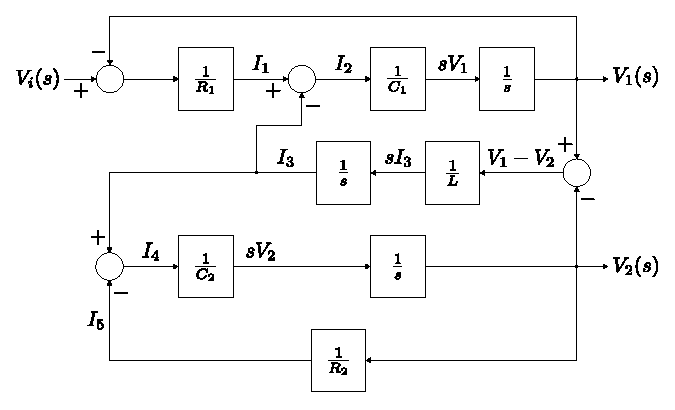
\includegraphics[scale=0.8]{cap2_fig1.eps}
	\caption{Legenda com citação \cite{Lipsum08}.}
	\label{fig:exemplo1}
\end{figure}
\end{verbatim}

Este código produz a Figura~\ref{fig:exemplo1}. As figuras podem ser redimensionadas de uma forma absoluta através da opção \code{scale}, ou de forma relativa, e.g., à largura da área de texto da forma: \path{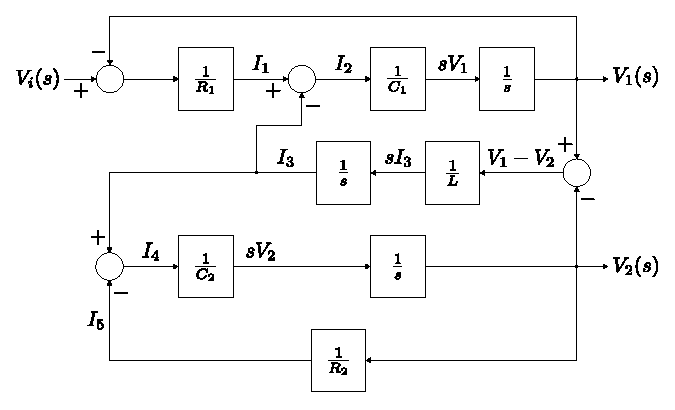
\includegraphics[width=0.5\textwidth]{cap2_fig1.eps}}. Se necessário pode também recorrer a sub-figuras (ver código deste ficheiro), como demonstrado pela Figura~\ref{fig:exemplo2} que contém as sub-figuras~\ref{fig:subfigA} e~\ref{fig:subfigB}.

\begin{figure}[htbp]
	\centering
	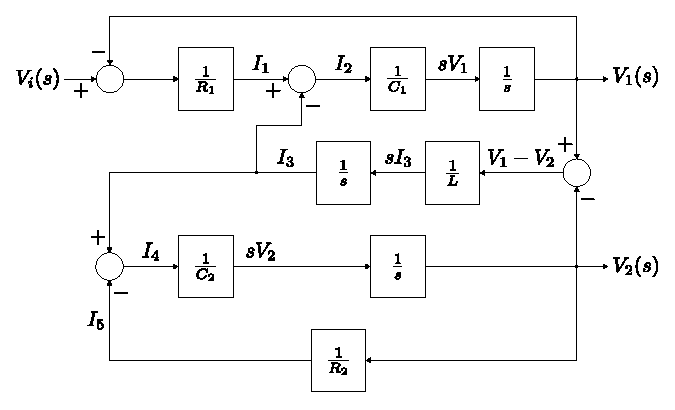
\includegraphics[scale=0.8]{cap2_fig1.eps}
	\caption{Legenda com citação \cite{Lipsum08}.}
	\label{fig:exemplo1}
\end{figure}

\begin{figure}[htbp]
  \centering
  \subcaptionbox{Uma sub-figura\label{fig:subfigA}}{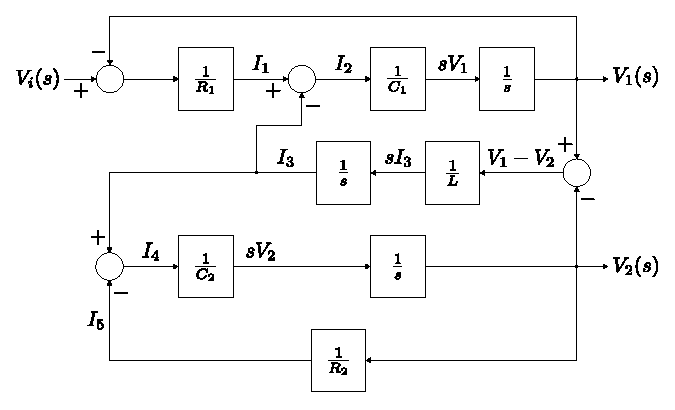
\includegraphics[width=0.45\linewidth]{cap2_fig1.eps}}
%  \hfill
  \subcaptionbox{\label{fig:subfigB}}{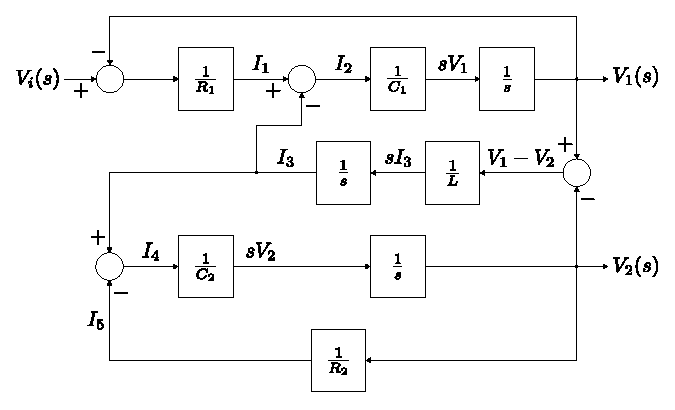
\includegraphics[width=0.45\linewidth]{cap2_fig1.eps}}
  \caption[Uma figura com duas sub-figuras.]{Uma figura com duas sub-figuras: (a) com legenda e (b) sem legenda.}
  \label{fig:exemplo2}
\end{figure}

Tenha em consideração que nem sempre as figuras irão aparecer no ponto onde escreveu o código, dado que o posicionamento depende do espaço disponível na página. Posicionar as figuras é trabalho para o \LaTeX{} e por isso só se deve preocupar em fazer as imagens, de preferência em formato vetorial (e.g., EPS, PDF). Neste sentido existem várias ferramentas, sendo o Inkscape (\url{inkscape.org}) uma excelente alternativa. O \LaTeX{} por omissão aceita os formatos PDF, JPG e PNG. As figuras devem ser sempre referidas no texto e devem também ter sempre uma legenda, definida através do comando \verb|\caption{}|. Não esquecer que quando uma figura é obtida de uma referência bibliográfica, i.e., não é da sua autoria, esse facto deve ser mencionado (ver legenda da Figura~\ref{fig:exemplo2}).

Este \textit{template} disponibiliza o comando adicional \verb|\inlinegraphics| que permite inserir figuras na linha de texto. Este é um exemplo \inlinegraphics{Inlinefigureexample.png}, verifique como usar o comando no código deste ficheiro. Por vezes uma figura necessita de ser apresentada em \textit{landscape}, onde a Figura~\ref{fig:exemplo3} é um exemplo desta forma de apresentação.

%%%%%%%%%%%%%%%%%%%%%%%%%%%%%%%%%%%%

\subsection{Tabelas}

As tabelas são uma forma importante de apresentação de informação. A Tabela~\ref{tab:basictable} ilustra a aplicação das principais diretrizes a ter em consideração na construção de tabelas:

\begin{enumerate}
   \item Não usar linhas verticais.
   \item A legenda é colocada antes da tabela.
   \item Usar as macros \verb|\toprule|, \verb|\midrule| e \verb|\bottomrule| para criar as linhas horizontais, respetivamente, do topo, meio e fundo da tabela.
\end{enumerate} 

\begin{landscape}
	\begin{figure}[htbp]
		\centering
		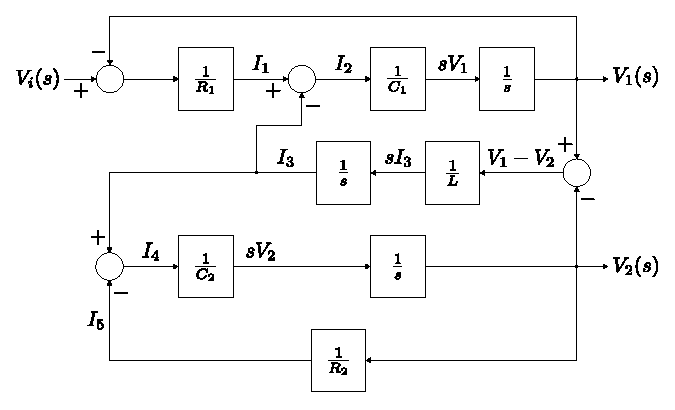
\includegraphics[scale=1.8]{cap2_fig1.eps}
		\caption{Uma figura em \textit{landscape}.}
		\label{fig:exemplo3}
	\end{figure}
\end{landscape}

Considere o seguinte código usado para criar a Tabela~\ref{tab:basictable}:

{\small
\begin{verbatim}
\begin{table}
\caption{Exemplo de uma tabela simples em \LaTeX{}.}
\label{tab:basictable}
\centering
	\begin{tabular}{l c c}
	\toprule
	\tabhead{Coluna 1} & \tabhead{Coluna 2} & \tabhead{Coluna 3} \\
	\midrule
	Linha 1 & 0.2 & 0.8\\
	Linha 2 & 0.17 & 0.7\\
	Linha 3 & 0.24 & 0.75\\
	Linha 4 & 0.68 & 0.3\\
	\bottomrule
\end{tabular}
\end{table}
\end{verbatim}
}

\begin{table}[htb]
	\caption{Exemplo de uma tabela simples em \LaTeX{}.}
	\label{tab:basictable}
	\centering
	\begin{tabular}{l c c}
	\toprule
	\tabhead{Coluna 1} & \tabhead{Coluna 2} & \tabhead{Coluna 3} \\
	\midrule
		Linha 1 & 0.2 & 0.8\\
		Linha 2 & 0.17 & 0.7\\
		Linha 3 & 0.24 & 0.75\\
		Linha 4 & 0.68 & 0.3\\
	\bottomrule
	\end{tabular}
\end{table}

Para fazer referência a tabelas use o comando \verb|\ref{<label>}|, onde  \verb|<label>| se refere ao rótulo definido por \verb|\label{<label>}|. Regra geral coloque sempre um til, i.e., \verb|Tabela~\ref{<label>}|, para introduzir um \textit{unbreakable space}. Ambientes e comandos adicionais podem ser empregues para construir tabelas mais complexas/específicas (desde que mantidas as regras gerais definidas anteriormente): \verb|tabularx|, \verb|longtable|, \verb|\multicolumn|, \verb|\multirow|, entre outros. Em caso de dificuldade na criação do código para as tabelas, sugere-se o \textit{website} \url{www.tablesgenerator.com}.

%%%%%%%%%%%%%%%%%%%%%%%%%%%%%%%%%%%%

\subsection{Listagens de código}

Para apresentar excertos de código-fonte no seu relatório este \textit{template} usa o \gls{pack} \verb|listings|. Tenha em consideração que por omissão as listagens estão definidas como flutuantes para que o \LaTeX{} as possa posicionar da melhor forma. Esta definição implica também que uma listagem não será dividida por uma nova página, pelo que é recomendado que utilize excertos que não excedam uma página. Existem muitas opções que podem ser especificadas neste ambiente, para mais informações consultar \url{en.wikibooks.org/wiki/LaTeX/Source_Code_Listings}.

O comando \verb|\printlistoflistings|, invocado no ficheiro \path{4_frontmatterlists.tex}, cria a secção ``Listagens'' no seu documento. Assim, se não necessitar de usar listagens deverá comentar este comando. A Listagem~\ref{lst:examplo1} e a Listagem~\ref{lst:examplo2} são dois exemplos de listagens de código. Analise o conteúdo deste ficheiro para mais detalhes.

\begin{center}
\begin{minipage}{0.7\linewidth}
\begin{lstlisting}[language=C, caption=Exemplo simples de C., label=lst:examplo1]
#include<stdio.h>
main()
{
	printf("Hello World");
}
\end{lstlisting}
\end{minipage}
\end{center}

Uma listagem de código também pode ser inserida diretamente de um ficheiro através do comando \verb|\lstinputlisting[<settings>]{<pathtofile>/file.c}|.

\begin{minipage}{0.9\linewidth}
\begin{lstlisting}[language=Python, caption=Exemplo longo em Python., label=lst:examplo2]
import numpy as np
    
def incmatrix(genl1,genl2):
    m = len(genl1)
    n = len(genl2)
    M = None #to become the incidence matrix
    VT = np.zeros((n*m,1), int)  #dummy variable
    
    #compute the bitwise xor matrix
    M1 = bitxormatrix(genl1)
    M2 = np.triu(bitxormatrix(genl2),1) 

    for i in range(m-1):
        for j in range(i+1, m):
            [r,c] = np.where(M2 == M1[i,j])
            for k in range(len(r)):
                VT[(i)*n + r[k]] = 1;
                VT[(i)*n + c[k]] = 1;
                VT[(j)*n + r[k]] = 1;
                VT[(j)*n + c[k]] = 1;
                
                if M is None:
                    M = np.copy(VT)
                else:
                    M = np.concatenate((M, VT), 1)               
                VT = np.zeros((n*m,1), int)  
    return M
\end{lstlisting}
\end{minipage}

%%%%%%%%%%%%%%%%%%%%%%%%%%%%%%%%%%%%

\subsection{Equações}

Se a sua tese fizer uso de conteúdo matemático, então a opção de usar o \LaTeX{} foi a mais acertada. O livro ``Uma não tão pequena introdução ao \LaTeX{}'' tem informação suficiente para a maioria dos casos de composição matemática, mas para conteúdos mais completos recomenda-se o guia \url{tug.ctan.org/info/short-math-guide/short-math-guide.pdf}. Adicionalmente, uma extensa lista de símbolos pode ser consultada em \url{tug.ctan.org/info/symbols/comprehensive/symbols-a4.pdf}.

O \LaTeX{} permite a escrita de equações \textit{inline} como $E = mc^{2}$ ou em modo \textit{display}, sendo neste caso  automaticamente numeradas:

\begin{verbatim}
\begin{equation}
	E = mc^{2} .
	\label{eqn:einstein}
\end{equation}
\end{verbatim}

\noindent que produz a famosa equação:

\begin{equation}
E = mc^{2} .
\label{eqn:einstein}
\end{equation}

Alternativamente, se pretender que (\ref{eqn:einstein}) não seja numerada pode usar o código \verb|$$ E = mc^{2} $$| que produz:
$$ E = mc^{2} .$$

%%%%%%%%%%%%%%%%%%%%%%%%%%%%%%%%%%%%

\subsection{Teoremas}

Teoremas, lemas e corolários devem ser numerados por ordem crescente. O \textit{template} fornece estes ambientes adaptados ao idioma selecionado para o documento em \file{main.tex}. Através do comando \verb|\newtheorem| pode criar ambientes adicionais do mesmo tipo (no ficheiro \file{preamble.tex}). 

\begin{theorem}
Isto é um exemplo da aplicação do ambiente \code{theorem}. Os teoremas são numerados por ordem crescente, iniciando em 1.
\end{theorem}

\begin{corollary}
Isto é um exemplo da aplicação do ambiente \code{corollary}. Os corolários são numerados por ordem crescente, iniciando em 1.
\end{corollary}

\begin{lemma}
Isto é um exemplo da aplicação do ambiente \code{lemma}. Os lemas são numerados por ordem crescente, iniciando em 1.
\end{lemma}

%%%%%%%%%%%%%%%%%%%%%%%%%%%%%%%%%%%%
\clearpage
\section{Notas Adicionais}

\textbf{Boa sorte!}

		
%\chapter{Ballerina}	%The main chapter title
\chaptermark{Ballerina}	%Short version for page header. Comment if not needed
\label{Chapter3}

Neste capitulo será explorado a linguagem de programação \textit{Ballerina}. Será feita uma introdução a mesma, enumerando as características distintivas, bem como é estruturado um projeto, como é construir, testado e implementado um serviço \textit{web}.

\section{Apresentação}

\textit{Ballerina}, é uma linguagem \textit{open source}, projetada pela empresa \ac{wso2} e que teve o seu lançamento no ano de 2019, visa facilitar o desenvolvimento de aplicações modernas baseadas em nuvem, ou seja, serviços altamente escaláveis e orientados a conexão. Apresenta várias semelhanças, com as linguagens C, C++, Java e JavaScript.

\textit{Ballerina} não é só uma linguagem de programação, mas sim um ecossistema, esta disponibiliza também um repositório no qual, este contém vários pacotes oficiais como pacotes feitos pela comunidade, que podem ser utilizados pelos desenvolvedores para facilitar a implementação de um certo problema, como, por exemplo, \textit{drivers} de bases de dados, autenticação, criptografia, entre outros. Também é uma maneira dos desenvolvedores poderem, gerir versões, verificar alterações nos pacotes e resolver conflitos de dependências entre pacotes. A esse repositório é-lhe dado o nome de \textit{Ballerina Central} \cite{centralBallerina}.

\section{Características}

Sendo que, \textit{Ballerina} recorre a um modelo de recorrência baseado em mensagens, cada serviço é executado simultaneamente, dado que, cada um deles é executado num processo.

Outra das suas caraterísticas é que esta é estaticamente tipada, o que significa que o tipo de uma variável é determinado em tempo de compilação e permanece o mesmo durante a execução do programa. Isso permite a capacidade de identificar problemas durante a compilação, o que pode reduzir o tempo e evitar que ocorram problemas durante a execução do programa. Por exemplo, se uma variável tiver sido definida como um inteiro e tentarmos atribuir-lhe uma \textit{string}, o compilador indicará um erro durante a compilação e não durante a execução \cite{tiposBallerina}.

Em \textit{Ballerina}, os dados são tratados como os outros tipos de dados funcionais como \textit{strings} e inteiros, dado que, são-lhes concedidos a mesma importância, permitindo que os desenvolvedores os manipulem e criem sem grande esforço. Uma das formas de isso ser obtido é mediante tipos de dados compostos como registos e objetos, aliados aos recursos de manipulação dos mesmos, como mapeamentos e filtros, que ajudam a processar um conjunto de informações grandes de forma eficiente e eficaz.

Comparando com outras linguagens, tem uma particularidade, no qual, é possível por meio de fluxogramas visualizar e a compreender o fluxo de dados num programa. Por outro lado, também pode servir para se entender como é feita a comunicação entre serviços.

E por último, tem suporte nativo com os formatos \textit{JSON} e \textit{XML}. \cite{ballerina}

\section{Estrutura de um projeto}
Um projeto em \textit{Ballerina} é organizado numa única unidade compartilhável denominada pacote. Por sua vez, um pacote pode ser constituído por vários módulos. Cada módulo é um conjunto de ficheiros do código-fonte, testes e recursos. É comum um projeto pequeno só ter um, mas à medida que o projeto vai ficando mais complexo nasce a necessidade de se criar mais, para melhor organizar o código e separar responsabilidades. Vale a pensa mencionar que cada ficheiro desta linguagem é acompanhado por uma extensão \textit{.bal} \cite{organizacaoCodigo}. Na figura \ref{fig:estruturaProjeto} é demonstrado um exemplo simples daquilo que foi mencionado em cima. 

\begin{figure}[H]
	\centering
	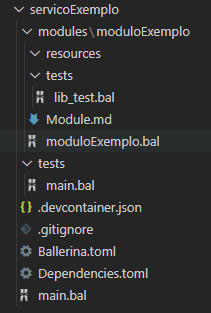
\includegraphics[scale=0.8]{estruturaProjeto}
	\caption{Exemplo da estrutura de um projeto.}
	\label{fig:estruturaProjeto}
\end{figure}

\section{Suporte num \ac{ide}}

O ambiente de desenvolvimento aconselhado para o desenvolvimento de código \textit{Ballerina} é o \ac{vsc}, dado, a sua integração nativa com a linguagem. Adicionalmente, esta disponibiliza uma extensão que auxilia o programador no desenvolvimento de código, uma vez que, disponibiliza funcionalidades tais como, correção de erros, \textit{noteboooks}, preenchimento automático de código e representação gráfica do código \cite{addon}.

\section{Implementar serviços na \textit{cloud}}
Feito o código necessário, este precisa de passar por um processo de implementação para passar a produção e começar a ser usado pelo utilizador final do sistema. Esse programa pode ser implementado na \textit{cloud} por meio de contentores \textit{docker} ou \textit{kubernetes}, para gerir e escalar os serviços em nuvens públicas ou privadas. Este processo descrito anteriormente, pode ser automatizado e simplificado com os recurso disponibilizados da linguagem, facilitando desta forma, o processo de implementação num ambiente de produção e fazendo com que, os desenvolvedores se concentrem mais a desenvolver os serviços do que com a implementação desses mesmos \cite{codeCloud}.

\section{Exemplos}
\subsection{Criação de um serviço}

Na Listagem \ref{lst:examplo1}, o código descrito importa o módulo \textit{HTTP}, que contém as funções para encarregar-se com pedidos \textit{HTTP}. Posteriormente, é criado um serviço que ouve pedidos na porta 9090 e na qual contém uma função do tipo \textit{GET} com o nome \textit{greeting} e que retorna uma \textit{string} \textit{"Hello, World"}.

\begin{minipage}{0.9\linewidth}
\begin{lstlisting}[language=ballerina, caption=Exemplo de um serviço. \cite{exemploB1}, label=lst:examplo1]
import ballerina/http;

service on new http:Listener(9090) {
    resource function get greeting() returns string {
        return "Hello, World!";
    }
}
\end{lstlisting}
\end{minipage}

\subsection{Conexão à base de dados}

Na Listagem \ref{lst:examplo4}, o código descrito importa o módulo \textit{MySQL} que contém funções que permitem o acesso a uma base de dados. Posteriormente é inicializado um cliente MySQL com as configurações necessárias, o anfitrião, o nome de utilizador, a palavra-passe e a porta. É importante mencionar que estes dados deveriam estar num ficheiro à parte e no qual seriam chamados. Para realizar isso seria preciso criar um ficheiro com o nome \textit{Config.toml} \cite{v}. 

Já na função \textit{init()}, nesta é instanciado um novo cliente MySQL, cujo objetivo é criar uma base de dados através da função \textit{execute()} com a respetiva \textit{query}. Ao criar-se a base de dados, já é possível criar-se uma tabela, visto isso, é utilizada outra instância já declarada anteriormente para interagir com a base de dados e executar comandos SQL na mesma. A tabela criada tem duas colunas, \textit{ingredient\_id} (declarado como inteiro, é a chave primária e incrementa automaticamente) e \textit{designation} (declarado como string).

\begin{minipage}{0.9\linewidth}
\begin{lstlisting}[language=ballerina, caption=Exemplo de uma coneção a base de dados. , label=lst:examplo4]
import ballerinax/mysql;
import ballerinax/mysql.driver as _; 
import ballerina/sql;

string USER = "myUser";
string PASSWORD = "myPassword";
string HOST = "localhost";
int PORT = 3306;

final mysql:Client dbClient;

function init() returns error? {
    mysql:Client dbClientCreate = check new(host=HOST, user=USER, password=PASSWORD, port=PORT);
    sql:ExecutionResult _ = check dbClientCreate->execute(`CREATE DATABASE IF NOT EXISTS Ingredient`);
    check dbClientCreate.close();
    dbClient = check new(host=HOST, user=USER, password=PASSWORD, port=PORT, database="Ingredient"); 
    sql:ExecutionResult _ = check dbClient->execute(`CREATE TABLE IF NOT EXISTS Ingredient.Ingredients (
                    ingredient_id INT AUTO_INCREMENT,
                    designation VARCHAR(255), 
                    PRIMARY KEY (ingredient_id)
                                         )`);                                
}
\end{lstlisting}
\end{minipage}

\subsection{Uso do \textit{RabbitMQ}}

Na Listagem \ref{lst:examplo5}, o código descrito importa o módulo \textit{RabbitMQ} que contém funções que permitem realizar a comunicação entre serviços.

Na função \textit{main()} é instanciado um novo cliente \textit{RabbitMQ}, no qual, são definidas o \textit{host} e porta de acesso ao servidor. E finalmente através da função \textit{queueDeclare} é criada uma \textit{queue} com o nome \textit{"TestQueue"}.

\begin{minipage}{0.9\linewidth}
\begin{lstlisting}[language=ballerina, caption=Exemplo de criação de uma queue. , label=lst:examplo5]
import ballerinax/rabbitmq;

public function main() returns error? {
    rabbitmq:Client client = check new (rabbitmq:DEFAULT_HOST, rabbitmq:DEFAULT_PORT);
    check client->queueDeclare("TestQueue");
}
\end{lstlisting}
\end{minipage}

Na Listagem \ref{lst:examplo6}, como na listagem anterior, importa o módulo \textit{RabbitMQ} e o módulo \textit{HTTP}. O presente código é um exemplo de como combinar um serviço \textit{web} com \textit{RabbitMQ}. Começa-se por declarar um registo \textit{"Test"}, que descreve um objeto, será este o objeto enviado na mensagem para o servidor. Depois disso é feita a declaração do serviço juntamente da porta em que ouvirá os pedidos. Dentro deste são instanciados um cliente \textit{RabbitMQ} e descritas duas funções. A  função \textit{"init"} é usada para inicializar uma conexão com o servidor, e a função \textit{"tests"} é responsável por receber o pedido do cliente \textit{web} e publicá-lo na \textit{queue} \textit{"TestQueue"} criada anteriormente na listagem \ref{lst:examplo5}.

\begin{minipage}{0.9\linewidth}
\begin{lstlisting}[language=ballerina, caption=Exemplo de publicação de mensagem para o servidor. , label=lst:examplo6]
import ballerina/http;
import ballerinax/rabbitmq;

type Test readonly & record {
    int id;
    string name;
};

service / on new http:Listener(9092) {
    private final rabbitmq:Client client;
    function init() returns error? {
        self.client = check new (rabbitmq:DEFAULT_HOST, rabbitmq:DEFAULT_PORT);
    }
    resource function post tests(Test test) returns http:Accepted|error {
        check self.client->publishMessage({
            content: test,
            routingKey: "TestQueue"
        });

        return http:ACCEPTED;
    }
}
\end{lstlisting}
\end{minipage}

Na Listagem \ref{lst:examplo7}, como na listagem anterior, importa o módulo \textit{RabbitMQ} e o módulo \textit{Log}. Começa-se por declarar um registo \textit{"Test"}, que descreve um objeto, será este o objeto recebido na mensagem enviada pelo servidor. 

Na função \textit{main()} é declarado um novo cliente \textit{RabbitMQ} com o \textit{host} e porta de acesso ao servidor. A seguir, a mensagem enviada é consumida através da função \textit{consumePayload()} da \textit{queue} \textit{"TestQueue"}. Depois do objeto \textit{"Test"} ser validado, uma mensagem aparecerá na consola devido à função \textit{"printInfo"} disponibilizada pelo módulo \textit{Log}.

\begin{minipage}{0.9\linewidth}
\begin{lstlisting}[language=ballerina, caption=Exemplo da consumição de uma mensagem do servidor. , label=lst:examplo7]
import ballerina/log;
import ballerinax/rabbitmq;

public type Test record {
    int id;
    string name;
};

public function main() returns error? {
    rabbitmq:Client client = check new (rabbitmq:DEFAULT_HOST, rabbitmq:DEFAULT_PORT);
    Test 'test = check client->consumePayload("TestQueue");
    if 'test.isValid {
        log:printInfo(string `Received valid test for ${'test.name}`);
    }
}
\end{lstlisting}
\end{minipage}

\subsection{Concorrência}

Na Listagem \ref{lst:examplo2}, o código descrito importa o módulo \textit{io}, que contém módulos de interação com ficheiros e módulos de \textit{output} e \textit{input}. É definido um registo com o nome \textit{"Person"} com dois campos, \textit{"name"} e \textit{"employed"} sendo os seus tipos, \textit{string} e \textit{boolean}, respetivamente. Também define uma função chamada \textit{"process"} que recebe dois parâmetros, uma lista de objetos \textit{"Person"} com o nome \textit{"members"} e uma lista de inteiros com o nome \textit{"quantities"}.

Na função descrita referida anteriormente, esta utiliza dois \textit{workers} para processar os dados recebidos como parâmetros na função. No caso do \textit{worker} com denominação "w1" é feito uma contagem dos membros empregado através do parâmetro \textit{"employed"} de cada objeto \textit{"Person"} na lista \textit{"members"}, essa contagem é envida a seguir para o \textit{worker} com denominação "w2" através do uso da ação (->) e conclui enviando um mensagem do tipo \textit{string} para o \textit{endpoint} da função com o valor contabilizado. Por outro lado, no w2, é inicialmente feito a soma de todos os valores recebidos no parâmetro \textit{"quantities"} e fica a espera do resultado retornado pelo "w1", recorrendo a ação (<-), dado esse recebimento, é a seguir calculado a média para os membros empregados e conclui enviando um mensagem do tipo \textit{string} para o \textit{endpoint} da função com esse valor calculado.

Após a definição do "w1" e "w2", a função fica à espera dos valores de cada \textit{worker} e imprime-as usando a função \textit{io:println}.

\begin{minipage}{0.9\linewidth}
\begin{lstlisting}[language=ballerina, caption=Exemplo de concorrência. \cite{exemploB2}, label=lst:examplo2]
import ballerina/io;

type Person record {|
    string name;
    boolean employed;
|};

function process(Person[] members, int[] quantities) {
    worker w1 {
        Person[] employedMembers = from Person p in members
            where p.employed
            select p;
        int count = employedMembers.length();
        count -> w2;
        string `Employed Members: ${count}` -> function;
    }
    worker w2 {
        int total = int:sum(...quantities);
        int employedCount = <- w1;
        int avg = employedCount == 0 ? 0 : total / employedCount;
        string `Average: ${avg}` -> function;
    }
    string x = <- w1;
    io:println(x);
    string y = <- w2;
    io:println(y);
}
\end{lstlisting}
\end{minipage}

\subsection{Testes de código}

Na Listagem \ref{lst:examplo3}, o código descrito importa o módulo \textit{test}, que contém módulos que possibilitam a realização de testes ao código feito. Uma função chamada \textit{"intAdd"} é definida com dois parâmetros, a e b, ambos inteiros, e retorna a soma dos valores inteiros. E outra função chamada \textit{"intAddTest"} é definida com a anotação \textit{"@test:Config"}, que especifica a configuração para a função de teste, para testar a função anteriormente construida. Através da função \textit{"test:assertEquals"} é possível comparar o retorna da função com o resultado esperado.


\begin{minipage}{0.9\linewidth}
\begin{lstlisting}[language=ballerina, caption=Exemplo de um teste desenvolvido. \cite{exemploB3}, label=lst:examplo3]
import ballerina/test;

public function intAdd(int a, int b) returns (int) {
    return a + b;
}

@test:Config {}
function intAddTest() {
    test:assertEquals(intAdd(1, 3), 4);
}
\end{lstlisting}
\end{minipage}

\section{Alternativas à linguagem}

As alternativas à linguagem em estudo para a construção de microsserviços são diversas. Algumas necessitam de recorrer a módulos externos para o desenvolvimento dos mesmos, enquanto outras através dos seus módulos nativos conseguem desenvolver estes sem necessitarem de importar módulos externos. Alguns exemplos são:
\begin{itemize}
    \item \textit{Java} recorrendo a \textit{Spring Boot} \cite{springBoot}
    \item \textit{Python} recorrendo a \textit{Flask} \cite{flask} ou \textit{Django} \cite{django}
    \item \textit{Node.js} recorrendo a \textit{Express.js} \cite{express} ou \textit{Fastify.js} \cite{fastify}
    \item \textit{Rust} recorrendo a \textit{Actix-web} \cite{actix}
    \item \textit{C\#} tem módulos nativos para o desenvolvimento de microsserviços \cite{csharp}
    \item \textit{Go} recorrendo \textit{Fiber} \cite{fiber}
\end{itemize}

	% Uncomment the lines as you write the chapters,
								% where 'chapter3' refers to a file chapter3.tex
%...							% in the 'chapters' folder
								
\chapter{Implementação}	%The main chapter title
\chaptermark{Implementação}	%Short version for page header. Comment if not needed
\label{Chapter6}

Neste capitulo será descrita como a solução foi implementada, referindo os vários microsserviços e as aplicações de deteção de linguagem. Finalmente será feita uma lista das tecnologias e ferramentas usadas para realização deste protótipo.


\section{Distribuição da aplicação}
A Tabela \ref{table:distribuicaoAplicacao} descreve a atribuição dos portos de cada um dos integrantes do sistema. 

\begin{table}[H]
\caption{Distribuição da aplicação}
\label{table:distribuicaoAplicacao}
\begin{center}
\begin{tabular}{ |p{5cm}|p{5cm}|  }
\hline
\textbf{Descrição} & \textbf{Porto} \\
\hline
SandwichService & 8091\\
\hline
IngredientService &  8090\\
\hline
ReviewService &  8095\\
\hline
StoreService &  8093\\
\hline
OrderService &  8094\\
\hline
CustomerService &  8092\\
\hline
LanguageDectetionService &  5000\\
\hline
APIGateway &  8000\\
\hline
RabbitMQ &  5672\\
\hline
MySQLContainer & 3306\\
\hline
\end{tabular} 
\end{center}
\end{table}

\section{\textit{MySQL Container}}

A Figura \ref{fig:databases} enumera as bases de dados criadas para a aplicação recorrendo ao uso do \textit{software} \textit{Podman} que faz a gestão do \textit{container} de um servidor de base de dados \textit{MySQL}. As bases de dados criadas foram as seguintes:
\begin{itemize}
    \item \textit{Ingredients}: Armazena informações acerca dos ingredientes
    \item \textit{Orders}: Armazena informações acerca das encomendas
    \item \textit{Reviews}: Armazena informações acerca das críticas
    \item \textit{Sandwiches}: Armazena informações acerca dos sanduíches
    \item \textit{Stores}: Armazena informações acerca das lojas
    \item \textit{Users}: Armazena informações acerca dos utilizadores
\end{itemize}

\begin{figure}[H]
	\centering
	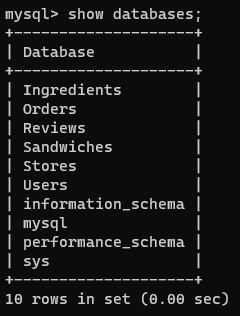
\includegraphics[scale=0.8]{databases.png}
	\caption{Bases de dados da aplicação}
	\label{fig:databases}
\end{figure}

\section{Variáveis do sistema}

As variáveis do sistema são argumentos (escritas em maiúsculas) definidos tipicamente num ficheiro à parte que podem ser acedidos pela aplicação. O uso destas variáveis é importante, dado que, podem esconder informações confidenciais, tais como, informações de acesso à base de dado e/ou informações repetitivas que podem ser reduzidas num argumento, como, por exemplo, \textit{URLs}. A Listagem \ref{lst:variavel1} apresenta os argumentos de acesso à base de dados guardados num ficheiro chamado \textit{Configuration.toml} com uma anotação no topo a referir o módulo que pode aceder aquela informação, que neste caso é o \textit{repository}.

\begin{minipage}{0.9\linewidth}
\begin{lstlisting}[language=python, caption=Definição de variáveis do sistema., label=lst:variavel1]
[ingredient.repository]
USER = "myUser"
PASSWORD = "myPassword"
HOST = "localhost"
PORT = 3306
\end{lstlisting}
\end{minipage}


Já no módulo \textit{repository}, surge o problema de como podemos aceder aos argumentos no ficheiro de configuração. Para isso é preciso recorrer à \textit{keyword configurable} que indica à aplicação que aquela variável tem que ter um valor igual ao valor do argumento com o mesmo nome no ficheiro de configuração, como pode ser visualizado na Listagem \ref{lst:variavel2}. Por isso é importante verificar-se a igualdade dos nomes para não haver variáveis que não tenham valor atribuído. 

\begin{minipage}{0.9\linewidth}
\begin{lstlisting}[language=python, caption=Invocação das variáveis do sistema., label=lst:variavel2]
configurable string USER = ?;
configurable string PASSWORD = ?; 
configurable string HOST = ?;
configurable int PORT = ?;
\end{lstlisting}
\end{minipage}

\section{Implementação dos microsserviços}
\subsection{\textit{Endpoints} do microsserviço Sanduíches}

Na Tabela \ref{table:endpoints1} são apresentados todos os \textit{endpoints} relativos ao microsserviço Sanduíche.

\begin{table}[H]
\caption{\textit{Endpoints} do microsserviço Sanduíche}
\label{table:endpoints1}
\begin{center}
\begin{tabular}{ |p{4cm}|p{6cm}|  }
\hline
\multicolumn{2}{|c|}{\textit{Endpoints}} \\
\hline
\textbf{Tipo de pedido} & \textbf{Endpoint}\\
\hline
POST & /sandwiches \\
\hline
GET & /sandwiches \\
\hline
GET & /sandwiches/searchById \\
\hline
POST & /sandwiches/descriptions \\
\hline
GET & /sandwiches/searchWithoutId \\
\hline
PUT & /sandwiches/state \\
\hline
PUT & /sandwiches/informations \\
\hline
\end{tabular} 
\end{center}
\end{table}


\subsection{\textit{Endpoints} do microsserviço Ingredientes}
Na Tabela \ref{table:endpoints2} são apresentados todos os \textit{endpoints} relativos ao microsserviço Ingredientes.

\begin{table}[H]
\caption{\textit{Endpoints} do microsserviço Ingredientes}
\label{table:endpoints2}
\begin{center}
\begin{tabular}{ |p{4cm}|p{6cm}|  }
\hline
\multicolumn{2}{|c|}{\textit{Endpoints}} \\
\hline
\textbf{Tipo de pedido} & \textbf{Endpoint}\\
\hline
POST & /ingredients \\
\hline
GET & /ingredients/searchById \\
\hline
GET & /ingredients/searchByDesignation \\
\hline
GET & /ingredients \\
\hline
PUT & /ingredients/state \\
\hline
GET & /ingredients/category \\
\hline
\end{tabular} 
\end{center}
\end{table}

\subsection{\textit{Endpoints} do microsserviço Críticas}
Na Tabela \ref{table:endpoints3} são apresentados todos os \textit{endpoints} relativos ao microsserviço Críticas.

\begin{table}[H]
\caption{\textit{Endpoints} do microsserviço Críticas}
\label{table:endpoints3}
\begin{center}
\begin{tabular}{ |p{4cm}|p{6cm}|  }
\hline
\multicolumn{2}{|c|}{\textit{Endpoints}} \\
\hline
\textbf{Tipo de pedido} & \textbf{Endpoint}\\
\hline
POST & /reviews \\
\hline
POST & /reviews/vote \\
\hline
GET & /reviews \\
\hline
GET & /reviews/reported \\
\hline
DELETE & /reviews/delete \\
\hline 
PUT & /reviews/report \\
\hline
PUT & /reviews/searchById \\
\hline
GET & /reviews/searchByClient \\
\hline
DELETE & /reviews/clientDeleteReview \\
\hline 
\end{tabular} 
\end{center}
\end{table}

\subsection{\textit{Endpoints} do microsserviço Lojas}
Na Tabela \ref{table:endpoints4} são apresentados todos os \textit{endpoints} relativos ao microsserviço Lojas.

\begin{table}[H]
\caption{\textit{Endpoints} do microsserviço Lojas}
\label{table:endpoints4}
\begin{center}
\begin{tabular}{ |p{4cm}|p{6cm}|  }
\hline
\multicolumn{2}{|c|}{\textit{Endpoints}} \\
\hline
\textbf{Tipo de pedido} & \textbf{Endpoint}\\
\hline 
POST & /stores \\
\hline
GET & /stores \\
\hline
GET & /stores/searchById \\
\hline
GET & /stores/searchByDesignation \\
\hline
GET & /stores/searchByAddress \\
\hline
DELETE & /stores/delete \\
\hline
PUT & /stores/closingHours \\
\hline
PUT & /stores/openingHours \\
\hline
\end{tabular} 
\end{center}
\end{table}

\subsection{\textit{Endpoints} do microsserviço Encomendas}
Na Tabela \ref{table:endpoints5} são apresentados todos os \textit{endpoints} relativos ao microsserviço Encomendas.

\begin{table}[H]
\caption{\textit{Endpoints} do microsserviço Encomendas}
\label{table:endpoints5}
\begin{center}
\begin{tabular}{ |p{4cm}|p{6cm}|  }
\hline
\multicolumn{2}{|c|}{\textit{Endpoints}} \\
\hline
\textbf{Tipo de pedido} & \textbf{Endpoint}\\
\hline
POST & /orders \\
\hline
GET & /orders/searchByStoreId \\
\hline
PUT & /orders/state  \\
\hline
PUT & /orders/seachByClientId \\
\hline
\end{tabular} 
\end{center}
\end{table}

\subsection{\textit{Endpoints} do microsserviço Clientes}
Na Tabela \ref{table:endpoints6} são apresentados todos os \textit{endpoints} relativos ao microsserviço Clientes.

\begin{table}[H]
\caption{\textit{Endpoints} do microsserviço Clientes}
\label{table:endpoints6}
\begin{center}
\begin{tabular}{ |p{4cm}|p{6cm}|  }
\hline
\multicolumn{2}{|c|}{\textit{Endpoints}} \\
\hline
\textbf{Tipo de pedido} & \textbf{Endpoint}\\
\hline
POST & /clients \\
\hline
GET & /clients/searchById \\
\hline
GET & /clients/searchByEmail \\
\hline
GET & /clients/searchByFiscalNumber \\
\hline
GET & /clients/authData/searchById \\
\hline
GET & /clients \\
\hline
POST & /clients/authData \\
\hline
POST & /clients/login \\
\hline
GET & /clients/data\\
\hline
\end{tabular} 
\end{center}
\end{table}

\subsection{\textit{Endpoint} do microsserviço de deteção de linguagem}
Na Tabela \ref{table:endpoints7} é apresentado o \textit{endpoint} relativos ao microsserviço de deteção de linguagem.

\begin{table}[H]
\caption{\textit{Endpoints} do microsserviço de deteção de linguagem}
\label{table:endpoints7}
\begin{center}
\begin{tabular}{ |p{4cm}|p{6cm}|  }
\hline
\multicolumn{2}{|c|}{Deteção de linguagem} \\
\hline
\textbf{Tipo de pedido} & \textbf{Endpoint}\\
\hline
POST & /language \\
\hline
\end{tabular} 
\end{center}
\end{table}

\section{API GATEWAY}

A criação de uma \textit{API GATEWAY} ajuda na implementação de segurança num certo sistema. Normalmente é utilizado em sistemas com uma arquitetura de microsserviços, no qual os vários serviços são independentes. Com este padrão de \textit{software}, os clientes podem interagir com os serviços por meio de uma interface única e unificada, dado que, os pedidos são encaminhados posteriormente para os respetivos serviços. Para além de algumas caraterísticas apresentadas anteriormente, este apresenta outras como, por exemplo:

\begin{itemize}
    \item Balanceamento de carga: Os pedidos podem ser distribuídos pelas várias instâncias
    \item Segurança: Criptógrafa o tráfego de dados e podem ser imposta políticas de segurança
    \item Limitação de taxa: Pode limitar o número de pedidos que um certo cliente pode fazer por um determinado tempo, garantindo desta forma que não haja sobrecargas ou ataques maliciosos
    \item Armazenamento em \textit{cache}: Pode armazenar em \textit{cache} respostas de serviços, levando a diminuição da latência e um aumento no desempenho
\end{itemize}

A Listagem \ref{lst:apiGateway} apresenta uma porção de código da \textit{API Gateway} desenvolvida. Para cada serviço que o sistema disponibiliza é necessária uma implementação semelhante ao código abaixo. Recorre-se a propriedade \textit{req.originalUrl} para obter-se o \textit{URL} do pedido original, por sua vez, é indispensável fazer a separação dos tipos de pedidos, dado que, no caso dos pedidos tipos \textit{GET} e \textit{DELETE}, este não precisam de um \textit{body}.

\begin{minipage}{1\linewidth}
\begin{lstlisting}[language=javascript, caption=API Gateway desenvolvida., label=lst:apiGateway]
app.all('/stores/*', (req, res) => {
    const serviceAUrl = `http://localhost:8093${req.originalUrl}`;
  
    if (req.method === 'GET' || req.method === 'DELETE') {
      axios({
        method: req.method,
        url: serviceAUrl,
        headers: req.headers
      })
        .then(response => {
          res.json(response.data);
        })
        .catch(error => {
          res.status(500).json({ error: 'An error occurred' });
        });
    } else {
      axios({
          method: req.method,
          url: serviceAUrl,
          headers: req.headers
        })
          .then(response => {
            res.json(response.data);
          })
          .catch(error => {
            res.status(500).json({ error: 'An error occurred' });
          });
    }
});
\end{lstlisting}
\end{minipage}

\section{Serviços de deteção de linguagem}

No que diz respeito a serviços de deteção de linguagem foram desenvolvidas duas aplicações recorrendo a diferentes tecnologias, como podem ser observados nas Listagens \ref{lst:python} e \ref{lst:nodejs}. Na primeira aplicação, Listagem \ref{lst:python}, foi utilizado o \textit{Python} com uma framework web denominada \textit{Flask}. Já na segunda aplicação, Listagem \ref{lst:nodejs},  foi utilizado o \textit{NodeJS} com uma framework web denominada \textit{Express.js}.

No primeiro exemplo é primariamente importado as classes \textit{Flask}, \textit{jsonify} e \textit{request} do módulo \textit{flask}, tal como, a função \textit{detect} do módulo \textit{langdetect}. Na linha a seguir é instanciado a classe \textit{Flask}. 

A seguir é definida uma rota \textit{/language} que invoca a função \textit{getLanguages()}. Quando a função for chamada a variável \textit{content} recebe os dados JSON e uma lista vazio é criada, de seguida, um \textit{loop} é utilizado, onde para cada um dos textos recebidos, é feita uma chamada à função \textit{detect}, que retorna a linguagem detetada e que é posteriormente adicionada a lista criada anteriormente para o efeito. Logo após a realização do \textit{loop} é criado um dicionário que contém as várias linguagens detetadas por ordem. Por fim, é retornado o dicionário convertido para uma resposta \textit{JSON}.

\begin{minipage}{0.9\linewidth}
\begin{lstlisting}[language=python, caption=Serviço de deteção de linguagem., label=lst:python]
from flask import Flask,jsonify,request
from langdetect import detect

app = Flask(__name__)


@app.route('/language', methods=['GET', 'POST'])
def getLanguage():
    content = request.json
    languages = []

    for text in content:
        language = detect(text["text"])
        languages.append(language)

    data = {
        "languages": languages
    }
    return jsonify(data)


if __name__ == '__main__':
    app.run()

\end{lstlisting}
\end{minipage}

Já no segundo exemplo é primariamente importado os módulos \textit{express} e \textit{languagedetect}, onde são posteriormente instanciados e no caso \textit{languagedetect} é definido o tipo de linguagem a ser apresentado. O funcionamento da obtenção das linguagens tem um esquema identifico ao referido no exemplo anterior. Sendo no final determinado o porto de funcionamento do servidor \textit{WEB}.

\begin{minipage}{0.9\linewidth}
\begin{lstlisting}[language=javascript, caption=Serviço de deteção de linguagem., label=lst:nodejs]
const express = require('express');
const app = express();
const LanguageDetect = require('languagedetect');
const lngDetector = new LanguageDetect();
lngDetector.setLanguageType("iso2");

app.use(express.json());

app.post('/language', (req, res) => {
    const content = req.body;
    let languages = [];

    content.forEach(text => {
        const language = lngDetector.detect(text.text,1);
        languages.push(language[0][0]);
    });

    data = {
        "languages":languages
    }

    res.json(data);
});

app.listen(5000, () => {
    console.log('Server running on port 5000');
});


\end{lstlisting}
\end{minipage}

Foram realizados testes com o \textit{software Postman} para verificar o funcionamento da aplicação de deteção de linguagem. Foi feito um pedido do tipo \textit{POST} ao \textit{URL http://127.0.0.1:5000/language} com uma lista de texto, um em português e outro em inglês. Ao qual foi recebido a lista das linguagens correta e na ordem correta, como se pode observar na Figura \ref{fig:testeDetecao}. Além disso, foi desenvolvido um teste de código para verificar o estado de saúde da aplicação \textit{WEB} ao longo do tempo que por sua vez que também foi bem sucedido, como se pode observar na Figura \ref{fig:testeDetecao1}.

\begin{figure}[H]
	\centering
	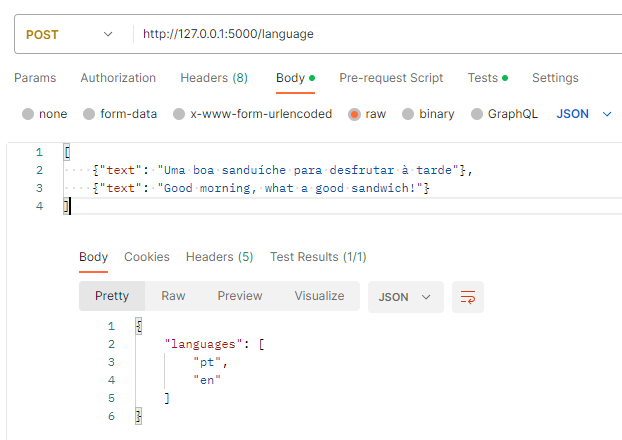
\includegraphics[scale=0.8]{testeDetecaoLinguagem.png}
	\caption{Pedido exemplo com retorno.}
	\label{fig:testeDetecao}
\end{figure}

\begin{figure}[H]
	\centering
	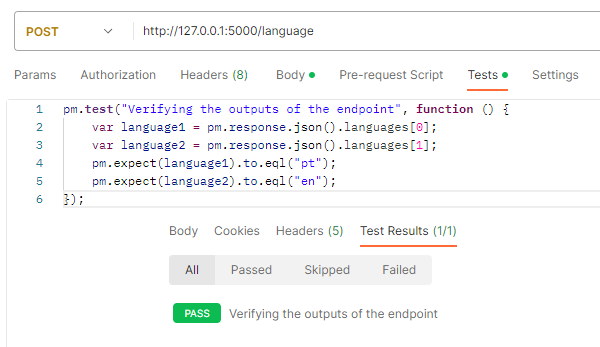
\includegraphics[scale=0.8]{testeDetecaoLinguagem1.png}
	\caption{Teste realizado ao pedido.}
	\label{fig:testeDetecao1}
\end{figure}

\section{Testes desenvolvidos}
\subsection{Teste unitário}

 apresenta um exemplo de um teste unitário desenvolvido no que diz respeito a criação de uma sanduíche. Começa-se por definir que esta porção de código é um teste com a anotação \textit{@test:Config {}}, as chavetas encontram-se vazias, dado que, não há configurações adicionais. Dado isso, é feita a invocação da função \textit{testSandwich()} que contém o código a ser executado. Essa função inicializa um o objeto \textit{SandwichDTO} com um exemplo de uma sanduíche que pode ser criada. Por fim, são feitas todas as verificações necessárias com a função \textit{assertEquals} do módulo \textit{test} para verificar se o objeto foi criado com as informações inseridas.

\begin{minipage}{1\linewidth}
\begin{lstlisting}[language=ballerina, caption=Exemplo de teste desenvolvido., label=lst:testeUnitario]
@test:Config {}
function testSandwich() {
    SandwichDTO sandwich = {designation: "Veggie Delight", selling_price: 5.99, 
        ingredients_id: [1, 2, 3], 
        descriptions: [{text: "A delicious vegetarian sandwich"}, 
                    {text: "Een heerlijk vegetarisch broodje"}]};
    test:assertEquals(sandwich.designation, "Veggie Delight");
    test:assertEquals(sandwich.selling_price, 5.99);
    test:assertEquals(sandwich.ingredients_id, [1, 2, 3]);
    test:assertEquals(sandwich.ingredients_id[0],1);
    test:assertEquals(sandwich.ingredients_id[1],2);
    test:assertEquals(sandwich.ingredients_id[2],3);
    test:assertEquals(sandwich.descriptions[0].text, "A delicious vegetarian sandwich");
    test:assertEquals(sandwich.descriptions[1].text, "Een heerlijk vegetarisch broodje");
    test:assertEquals(sandwich.descriptions.length(), 2);
    test:assertEquals(sandwich.ingredients_id.length(), 3);
}
\end{lstlisting}
\end{minipage}

\subsection{Testes de integração}

A Figura \ref{fig:testesPostman} apresenta um excerto dos testes de integração desenvolvidos para testar as funcionalidades de cada um dos serviços que fazem parte da logística do sistema. Estes forma realizados com o auxílio do \textit{software Postman}.

\begin{figure}[H]
	\centering
	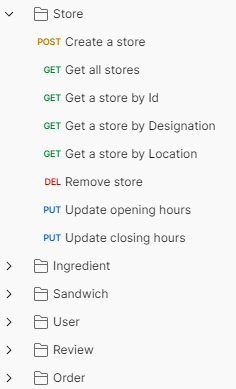
\includegraphics[scale=0.8]{figures/testesPostman.png}
	\caption{Testes desenvolvidos em Postman.}
	\label{fig:testesPostman}
\end{figure}

Já a Figura \ref{fig:testesPostman2}, nesta é demonstrado um exemplo de um \textit{script} criado, visando gerar dados que vão ser usados, neste caso, no pedido de criação de uma loja.

\begin{figure}[H]
	\centering
	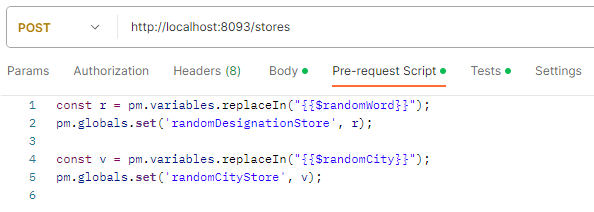
\includegraphics[scale=0.8]{figures/testesPostman2.png}
	\caption{Testes desenvolvidos em Postman.}
	\label{fig:testesPostman2}
\end{figure}

Por outro lado, a Figura \ref{fig:testesPostman1} apresenta um exemplo de testes efetuados no teste de integração. Nestes são feitos testes para verificar o código \textit{HTTP} e a presença de certos campos na resposta recebida. 

\begin{figure}[H]
	\centering
	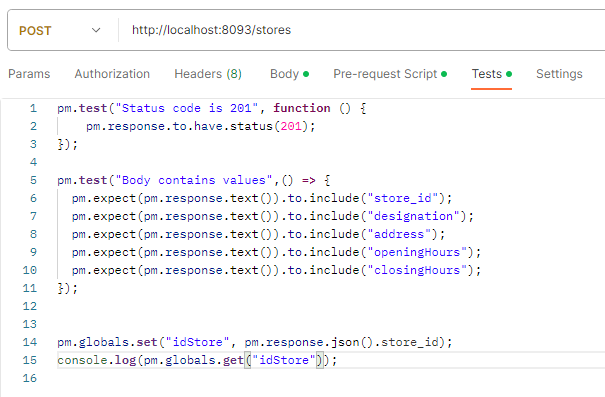
\includegraphics[scale=0.8]{figures/testesPostman1.png}
	\caption{Testes desenvolvidos em Postman.}
	\label{fig:testesPostman1}
\end{figure}

\subsection{Teste de desempenho e carga}

A Figura \ref{fig:testesCarga} apresenta testes de desempenho e carga desenvolvidos para comparar o atual desempenho do sistema com o requisito apresentado na secção Análise. Estes foram realizados com o auxílio do \textit{software JMeter}.

\begin{figure}[H]
	\centering
	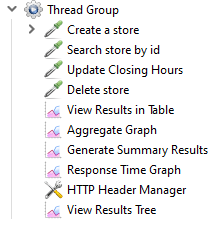
\includegraphics[scale=0.8]{figures/testesCarga.png}
	\caption{Testes de desempenho e carga.}
	\label{fig:testesCarga}
\end{figure}

Cada utilizador virtual executa o \textit{Thread Group}, este é composto por vários pedidos \textit{HTTP}, neste caso foram escolhidos um de cada tipo de pedido (\textit{POST}, \textit{GET}, \textit{PUT} e \textit{DELETE}). Este é constituído por parâmetros modificáveis, o número de utilizadores virtuais, o período de arranque e o número de vezes que o utilizador executará o mesmo. Vale a pena referir que o período de arranque representa o tempo necessário para que todos os utilizadores virtuais sejam adicionados à execução do teste.

Na Tabela \ref{table:desempenho} são apresentados vários cenários. Para cada cenário foram anotados os seguintes parâmetros:
\begin{itemize}
    \item Número de ciclos
    \item Utilizadores virtuais
    \item Taxa de transferência 
    \item Tempo decorrido
    \item Período de arranque utilizado
\end{itemize}

\begin{table}[H]
\caption{Testes de desempenho e carga}
\label{table:desempenho}
\begin{center}
\begin{tabular}{ |p{2.5cm}|p{2.5cm}|p{2.5cm}|p{2.5cm}|p{2.5cm}|  }
\hline
\multicolumn{5}{|c|}{Testes de desempenho e carga} \\
\hline
\textbf{Número de ciclos} & \textbf{Utilizadores virtuais} & \textbf{Taxa de transferência (pedidos por segundo)} & \textbf{Tempo decorrido (mm:ss.ms)} & \textbf{Período de arranque (s)}\\
\hline
1 & 10 & 232.6 & 00:00.102 & 0\\
\hline
1 & 100 & 341.0 & 00:01.230 & 1\\
\hline
1 & 1000 & 199.3 & 00:10.935 & 20\\
\hline
10 & 10 & 385.0 & 00:01.312 & 0\\
\hline
10 & 100 & 194.9 & 00:20.592 & 20\\
\hline
10 & 1000 & 332.3 & 02:00.744 & 60\\
\hline
\end{tabular} 
\end{center}
\end{table}

Para linha da tabela são apresentadas nas figuras abaixo (Figura \ref{fig:teste1}, Figura \ref{fig:teste2}, Figura \ref{fig:teste3}, Figura \ref{fig:teste4}, Figura \ref{fig:teste5} e Figura \ref{fig:teste6}) informações adicionais. Cada figura expõe a média, a mediana, o mínimo e o máximo para o número das amostras (total de pedidos realizados para cada pedido), com a adição do erro e a taxa de transferência. 

\begin{figure}[H]
	\centering
	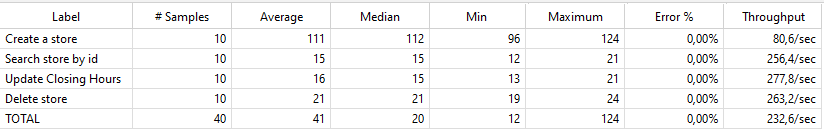
\includegraphics[scale=0.7]{figures/print1teste.png}
	\caption{Testes de desempenho e carga linha 1.}
	\label{fig:teste1}
\end{figure}
\begin{figure}[H]
	\centering
	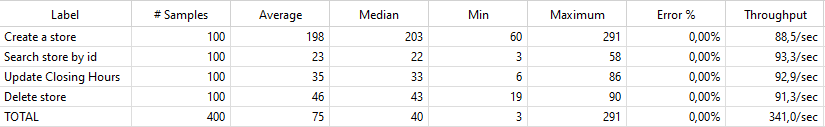
\includegraphics[scale=0.7]{figures/print2teste.png}
	\caption{Testes de desempenho e carga linha 2.}
	\label{fig:teste2}
\end{figure}

\begin{figure}[H]
	\centering
	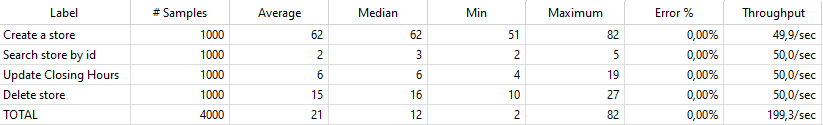
\includegraphics[scale=0.7]{figures/print3teste.png}
	\caption{Testes de desempenho e carga linha 3.}
	\label{fig:teste3}
\end{figure}

\begin{figure}[H]
	\centering
	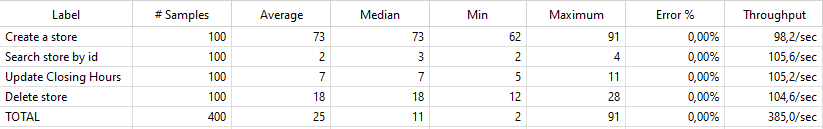
\includegraphics[scale=0.7]{figures/print4teste.png}
	\caption{Testes de desempenho e carga linha 4.}
	\label{fig:teste4}
\end{figure}

\begin{figure}[H]
	\centering
	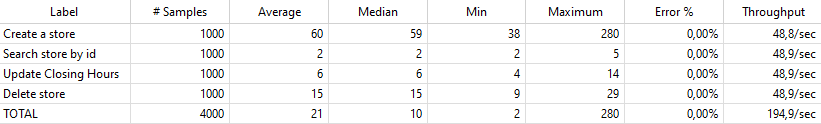
\includegraphics[scale=0.7]{figures/print5teste.png}
	\caption{Testes de desempenho e carga linha 5.}
	\label{fig:teste5}
\end{figure}

\begin{figure}[H]
	\centering
	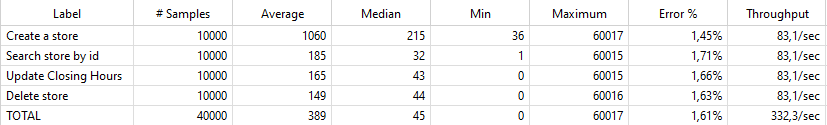
\includegraphics[scale=0.7]{figures/print6teste.png}
	\caption{Testes de desempenho e carga linha 6.}
	\label{fig:teste6}
\end{figure}

\section{Documentação da API}

Após realizada a implementação dos serviços procedeu-se a documentação dos mesmos. A Figura \ref{fig:documentacao} é um exemplo do como foi estruturada a informação para cada caso de uso. A documentação feita visa auxiliar os desenvolvedores/programadores a intenderem o funcionamento do sistema. Estes podem fornecer informações tais como:

\begin{itemize}
    \item Correspondente caso de uso
    \item O \textit{url do endpoint}
    \item Exemplo de pedido e resposta
    \item Parâmetros de consulta
    \item Possíveis respostas
\end{itemize}

\begin{figure}[H]
	\centering
	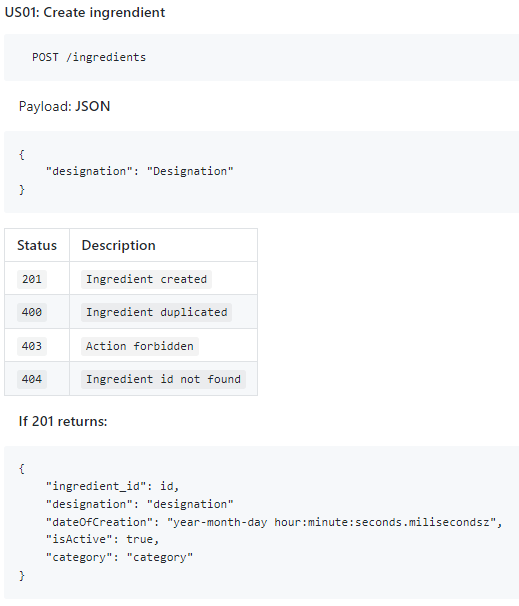
\includegraphics[scale=0.8]{figures/documentação.png}
	\caption{Documentação da API.}
	\label{fig:documentacao}
\end{figure}



\section{Tecnologias e ferramentas usadas}
Para a implementação desta solução foram usadas as seguintes tecnologias e ferramentas:

\begin{itemize}
    \item \textit{Ballerina}: Linguagem de programação
    \item \textit{MySQL}: Sistema de gestão de bases de dados
    \item \textit{Podman}: Plataforma de contentores
    \item \textit{Postman}: Ferramenta de teste para \textit{APIs}
    \item \textit{RabbitMQ}: Programa de mensagens
    \item \textit{Visual Studio Code}: Editor de código
\end{itemize}

%%%%%%%%%%%%%%%%%%%%%%%%%%%%%%%%%%%%%%%%%%%%%%%%%%%%%%%%%%%%%%%%%%%%%%%%%%%%%%%%%%%%%%%%%
% Print the bibliographic references using the ieeetr format from the 'sampleRefs.bib' file (root folder)

\printrefereces{sampleRefs}		% Change the 'sampleRefs' name to match your .bib file name,
								% a good option to make bib files is https://www.jabref.org/
%%%%%%%%%%%%%%%%%%%%%%%%%%%%%%%%%%%%%%%%%%%%%%%%%%%%%%%%%%%%%%%%%%%%%%%%%%%%%%%%%%%%%%%%%
\begin{appendices}
% Include the appendices of the document as separate files from the 'chapters' folder

% Appendix A

\chapter{Título do Anexo} % Main appendix title
\label{AppendixA} % For referencing this appendix elsewhere, use \ref{AppendixA}

%%%%%%%%%%%%%%%%%%%%%%%%%%%%%%%%%%%%%%%%%%%%%%%%%%%%%%%%%%%%%%%%%%%%%%%%%%%%%%%%%%
\section{Secção}

\lipsum[1]

%%%%%%%%%%%%%%%%%%%%%%%%%%%%%%%%%%%%%%%%%%%%%%%%%%%%%%%%%%%%%%%%%%%%%%%%%%%%%%%%%%
\section{Mais uma secção do Anexo~\ref{AppendixA}}

\lipsum[1]

	% Uncomment the lines as you write the appendices,
%\include{chapters/appendixB}	% or comment the lines if not used

\end{appendices}
%%%%%%%%%%%%%%%%%%%%%%%%%%%%%%%%%%%%%%%%%%%%%%%%%%%%%%%%%%%%%%%%%%%%%%%%%%%%%%%%%%%%%%%%%
\end{document}  
